% /*
%  * ----------------------------------------------------------------------------
%  * "THE BEER-WARE LICENSE" (Revision 42):
%  * Julian Klaiber and Severin Dellsperger wrote this file. As long as you retain this notice you
%  * can do whatever you want with this stuff. If we meet some day, and you think
%  * this stuff is worth it, you can buy us a beer in return.
%  * ----------------------------------------------------------------------------
%  */

% Template Informationen
\documentclass[
a4paper,
oneside,
10pt,
fleqn,
headsepline,
toc=listofnumbered, 
bibliography=totocnumbered]{scrartcl}

% deutsche Trennmuster etc.
\usepackage[T1]{fontenc}
\usepackage[utf8]{inputenc}
\usepackage[english, ngerman]{babel} % \selectlanguage{english} if  needed
\usepackage{lmodern} % use modern latin fonts

% Custom commands
\newcommand{\GITHUB}{https://github.com/jklaiber/HSR}
\newcommand{\LICENSEURL}{https://en.wikipedia.org/wiki/Beerware}
\newcommand{\LICENSE}{
"THE BEER-WARE LICENSE" (Revision 42):
Julian Klaiber and Severin Dellsperger wrote this file. As long as you retain this notice you
can do whatever you want with this stuff. If we meet some day, and you think
this stuff is worth it, you can buy us a beer in return.
}

% Jede Überschrift 1 auf neuer Seite
\let\stdsection\section
\renewcommand\section{\clearpage\stdsection}

% Multiple Authors
\usepackage{authblk}

% Include external pdf
\usepackage{pdfpages}

% Layout / Seitenränder
\usepackage{geometry}

% Inhaltsverzeichnis
\usepackage{makeidx} 
\makeindex

\usepackage{url}
\usepackage[pdfborder={0 0 0}]{hyperref}
\usepackage[all]{hypcap}
\usepackage{hyperxmp} % for license metadata

% Glossar und Abkürzungsverzeichnis
\usepackage[acronym,toc,nopostdot]{glossaries}
\setglossarystyle{altlist}
\usepackage{xparse}
\DeclareDocumentCommand{\newdualentry}{ O{} O{} m m m m } {
	\newglossaryentry{gls-#3}{
		name={#4 : #5},
		text={#5\glsadd{#3}},
		description={#6},
		#1
	}
	\makeglossaries
	\newacronym[see={[Siehe:]{gls-#3}},#2]{#3}{#4}{#5\glsadd{gls-#3}}
}
\makeglossaries

% Mathematik
\usepackage{amsmath}
\usepackage{amssymb}
\usepackage{amsfonts}
\usepackage{enumitem}

% Images
\usepackage{graphicx}
\graphicspath{{images/}} % default paths

% Boxes
\usepackage{fancybox}

%Tables
\usepackage{tabu}
\usepackage{booktabs} % toprule, midrule, bottomrule
\usepackage{array} % for matrix tables
\usepackage{multicol} %multicol

% Header and footer
\usepackage{scrlayer-scrpage}
\setkomafont{pagehead}{\normalfont}
\setkomafont{pagefoot}{\normalfont}
\automark*{section}
\clearpairofpagestyles
\ihead{\headmark}
\ohead{\AUTHOR}
\cfoot{\pagemark}

% Pseudocode
\usepackage{algorithmic}
\usepackage[linesnumbered,ruled]{algorithm2e}

% Code Listings
\usepackage{listings}
\usepackage{color}
\usepackage{beramono}

\definecolor{bluekeywords}{rgb}{0,0,1}
\definecolor{greencomments}{rgb}{0,0.5,0}
\definecolor{redstrings}{rgb}{0.64,0.08,0.08}
\definecolor{xmlcomments}{rgb}{0.5,0.5,0.5}
\definecolor{types}{rgb}{0.17,0.57,0.68}

\lstdefinestyle{visual-studio-style}{
	language=[Sharp]C,
	columns=flexible,
	showstringspaces=false,
	basicstyle=\footnotesize\ttfamily, 
	commentstyle=\color{greencomments},
	morekeywords={partial, var, value, get, set},
	keywordstyle=\bfseries\color{bluekeywords},
	stringstyle=\color{redstrings},
	breaklines=true,
	breakatwhitespace=true,
	tabsize=4,
	numbers=left,
	numberstyle=\tiny\color{black},
	frame=lines,
	showspaces=false,
	showtabs=false,
	escapeinside={£}{£},
}

\definecolor{DarkPurple}{rgb}{0.4, 0.1, 0.4}
\definecolor{DarkCyan}{rgb}{0.0, 0.5, 0.4}
\definecolor{LightLime}{rgb}{0.3, 0.5, 0.4}
\definecolor{Blue}{rgb}{0.0, 0.0, 1.0}

\lstdefinestyle{cevelop-style}{
	language=C++,  
	columns=flexible,
	showstringspaces=false,     
	basicstyle=\footnotesize\ttfamily, 
	keywordstyle=\bfseries\color{DarkPurple},
	commentstyle=\color{LightLime},
	stringstyle=\color{Blue}, 
	escapeinside={£}{£}, % latex scope within code      
	breaklines=true,
	breakatwhitespace=true,
	showspaces=false,
	showtabs=false,
	tabsize=4,
	morekeywords={include,ifndef,define},
	numbers=left,
	numberstyle=\tiny\color{black},
	frame=lines,
}

\lstdefinestyle{eclipse-style}{
	language=Java,  
	columns=flexible,
	showstringspaces=false,     
	basicstyle=\footnotesize\ttfamily, 
	keywordstyle=\bfseries\color{DarkPurple},
	commentstyle=\color{LightLime},
	stringstyle=\color{Blue}, 
	escapeinside={£}{£}, % latex scope within code      
	breaklines=true,
	breakatwhitespace=true,
	showspaces=false,
	showtabs=false,
	tabsize=4,
	morekeywords={length},
	numbers=left,
	numberstyle=\tiny\color{black},
	frame=lines,
}
\lstset{style=eclipse-style}



% Theorems \begin{mytheo}{title}{label}
\usepackage{tcolorbox}
\tcbuselibrary{theorems}
\newtcbtheorem[number within=section]{definiton}{Definition}%
{fonttitle=\bfseries}{def}
\newtcbtheorem[number within=section]{remember}{Merke}%
{fonttitle=\bfseries}{rem}
\newtcbtheorem[number within=section]{hint}{Hinweis}%
{fonttitle=\bfseries}{hnt}

% Colors
\definecolor{strings}{HTML}{448c25}
\definecolor{comments}{HTML}{aaaaaa}
\definecolor{keywords}{HTML}{aa3d8c}
\definecolor{background}{HTML}{f4f4f4}
\definecolor{numbers}{HTML}{a884e0}

% Default style
\lstdefinestyle{default}{
    backgroundcolor=\color{background},
    basicstyle=\ttfamily\small,
    breakatwhitespace=true,
    breaklines=true,
    commentstyle=\color{comments},
    deletekeywords={},
    escapeinside={}{},
    extendedchars=true,
    frame=lines,
    keepspaces=true,
    keywordstyle=\color{keywords},
    morekeywords={},
    numbers=left,
    numberstyle=\ttfamily\color{numbers},
    rulecolor=\color{numbers},
    showspaces=false,
    showstringspaces=false,
    showtabs=false,
    stepnumber=1,
    stringstyle=\color{strings},
    tabsize=2,
}
\lstset{
    style=default,
    columns=fullflexible
}

% Language cisco-config
\lstdefinelanguage{cisco-config}{
    morekeywords={no,ip,ipv6,int,interface},
    morecomment=[l][\color{comments}]{!},
    numbers=none
}

% Language cisco-teminal
\lstdefinelanguage{cisco-terminal}{
    morecomment=[l][\color{strings}]{\#},
    morecomment=[l][\color{strings}]{>},
    numbers=none
}

\lstdefinelanguage{bash}{
    numbers=none
}

\makeatletter
\@addtoreset{section}{part}
\makeatother

% Boxes
\tcbuselibrary{most}

\usepackage{fontawesome}

% \cmd{...}
\newcommand{\cmd}[1]{\texttt{#1}}

% Info Box
\definecolor{infobar}{HTML}{02cefc}
\definecolor{infobackground}{HTML}{baf0fc}
\newcommand{\info}[2]{
    \begin{tcolorbox}[
        arc = 0mm,
        boxrule = 0pt,
        breakable,
        before skip=11pt,
        before skip=11pt,
        title = \faInfo~#1,
        fonttitle = \sffamily\bfseries,
        coltitle = white,
        colbacktitle = infobar,
        colback = infobackground,
        toptitle=2mm,
        bottomtitle=2mm,
        top=4mm,
        bottom=4mm
    ]
    #2
    \end{tcolorbox}
}

% Warning Box
\definecolor{warnbar}{HTML}{f90053}
\definecolor{warnbackground}{HTML}{fcc4d7}
\newcommand{\warn}[2]{
    \begin{tcolorbox}[
        arc = 0mm,
        boxrule = 0pt,
        breakable,
        before skip=11pt,
        before skip=11pt,
        title = \faWarning~#1,
        fonttitle = \sffamily\bfseries,
        coltitle = white,
        colbacktitle = warnbar,
        colback = warnbackground,
        toptitle=2mm,
        bottomtitle=2mm,
        top=4mm,
        bottom=4mm
    ]
    #2
    \end{tcolorbox}
}

% Login Information Box
\definecolor{loginbar}{HTML}{FA8A05}
\definecolor{loginbackground}{HTML}{F3D4AF}
\newcommand{\login}[2]{
    \begin{tcolorbox}[
        arc = 0mm,
        boxrule = 0pt,
        breakable,
        before skip=11pt,
        before skip=11pt,
        title = \faKey~#1,
        fonttitle = \sffamily\bfseries,
        coltitle = white,
        colbacktitle = loginbar,
        colback = loginbackground,
        toptitle=2mm,
        bottomtitle=2mm,
        top=4mm,
        bottom=4mm
    ]
    #2
    \end{tcolorbox}
}

\definecolor{settingborder}{HTML}{0066CC}
\definecolor{settingcontent}{HTML}{E5F2FA}
\newcommand{\setting}[1]{
    \begin{tcolorbox}[
        colback = settingcontent,
        colframe = settingborder
    ]
    You can find the settings under: \\
    \textbf{\clicks{~#1}}
    \end{tcolorbox}
}

\definecolor{configurationborder}{HTML}{005700}
\definecolor{configurationcontent}{HTML}{e6ffcc}
\newcommand{\configuration}[2]{
    \begin{tcolorbox}[
        colback = configurationcontent,
        colframe = configurationborder
    ]
    \textbf{Configuration:}\\
    To reach an output like below you only have to add/change the following parameters 
    ~#1
    You can find the settings under: \\
    \textbf{\clicks{~#2}}
    \end{tcolorbox}
}


\usepackage{multirow}

% URLs
\urlstyle{rm}
\definecolor{link}{HTML}{0450f2}
\hypersetup{
    colorlinks,
    allcolors=.,
    urlcolor=link,
}

% \url[display]{url} or \url{url}
\renewcommand{\url}[2][]{%
    \ifstrempty{#1}{%
        \burlalt{#2}{#2}%
    }{%
        \burlalt{#1}{#2}%
    }%
}

% Clicks
\newcommand{\clicks}[1]{%
    $\foreach \n [count=\ni] in {#1}{%
        \ifnum\ni=1%
            \textit{\n}%
        \else%
            \rightarrow \textit{\n}%
        \fi%
    }$%
}

% Keystrokes
\newcommand{\keys}[1]{%
    $\foreach \n [count=\ni] in {#1}{%
        \ifnum\ni=1%
            \textit{\n}%
        \else%
            + \textit{\n}%
        \fi%
    }$%
}

% Dokumentinformationen
\newcommand{\INSTITUTE}{University of Applied Science Rapperswil}
\newcommand{\SUBJECT}{System Modelling and Simulation}
\newcommand{\TITLE}{Zusammenfassung inkl. Cheatsheet}
\newcommand{\AUTHORONE}{Severin Dellsperger}
\selectlanguage{german}

% Titelseite einfügen
% pdf metadata
\hypersetup{
	pdfauthor={\AUTHOR},
	pdftitle={\SUBJECT \TITLE},
	pdfcopyright={\LICENSE},
	pdflicenseurl={\LICENSEURL}
}

\begin{document}
	
\begin{titlepage}

\newcommand{\HRule}{\rule{\linewidth}{0.5mm}} % Defines a new command for the horizontal lines, change thickness here

\center % Center everything on the page
 
%----------------------------------------------------------------------------------------
%	HEADING SECTIONS
%----------------------------------------------------------------------------------------

\textsc{\LARGE \INSTITUTE}\\[1.5cm] % Name of your university/college
\textsc{\Large \SUBJECT}\\[0.5cm] % Major heading such as course name

%----------------------------------------------------------------------------------------
%	TITLE SECTION
%----------------------------------------------------------------------------------------

\HRule \\[0.6cm]
{ \huge \bfseries \TITLE}\\[0.4cm] % Title of your document
\HRule \\[1.5cm]

%----------------------------------------------------------------------------------------
%	AUTHOR SECTION
%----------------------------------------------------------------------------------------

\begin{minipage}{0.4\textwidth}
\begin{flushleft} \large
\emph{Author:}\\
\AUTHORONE % Your name
\end{flushleft}
\end{minipage}
~
\begin{minipage}{0.4\textwidth}
\begin{flushright} \large
\emph{} \\
\AUTHORTWO
\end{flushright}
\end{minipage}\\[2cm]

%----------------------------------------------------------------------------------------
%	DATE SECTION
%----------------------------------------------------------------------------------------

{\large \today}\\[2cm] % Date, change the \today to a set date if you want to be precise

%----------------------------------------------------------------------------------------
%	LOGO SECTION
%----------------------------------------------------------------------------------------


\includegraphics[width=10cm,height=5cm,keepaspectratio]{ressources/hsr_logo.jpg}\\[1cm] 
 
%----------------------------------------------------------------------------------------

\vfill % Fill the rest of the page with whitespace

\end{titlepage} 	


% Inhaltsverzeichnis einfügen
\tableofcontents
\newpage

% Start der Dokumentation

%Bild einfügen:
%\begin{minipage}[t]{1\textwidth}
%    \centering
%	\includegraphics[width=0.8\linewidth]{images/lab_10_physical_topology.png}
%\end{minipage}

\part{Zusammenfassung}
\section{Einführung und Grundlagen der Simulation}
\subsection{Objekte der Simulation}
\subsubsection{Simulation}
Unter Simulation versteht man Methoden und Anwendungen, um ein ein reales oder geplantes System zu imitieren oder nachzubilden.
\begin{center}
\textbf{Simulation ist eine experimentelle Methode!}
\end{center}
\subsubsection{System}
Ein System ist eine Einrichtung oder Prozess mit definierten Grenzen und Schnittstellen in einem gewissen (System-)Kontext. Es besteht aus diversen Systemkomponenten, wie beispielsweise Hardware, Software, Personen oder natürlichen/künstlichen Komponenten. Ebenfalls kann eine Systemkomponente wiederrum ein Subsystem sein.

Ein reales Problem/System wird auch als komplexes oder kybernetisches System bezeichnet:
\begin{itemize}
    \item \textbf{Komplexität} - Vielgestaligkeit - es gibt viele Systemkomponenten/Faktoren welche untereinander extrem vernetzt und verbunden sind und sich gegenseitig beeinflussen
 
    \item \textbf{Kompliziertheit} - Schwierigkeit -  schwierige/nicht verstandene Zusammenhänge und Faktoren
\item \textbf{Kybernetik} - Kommunikation und Regelung unabhängiger komplexer, komplizierter Systeme
\end{itemize}
   \begin{minipage}[t]{1\textwidth}
    \centering
	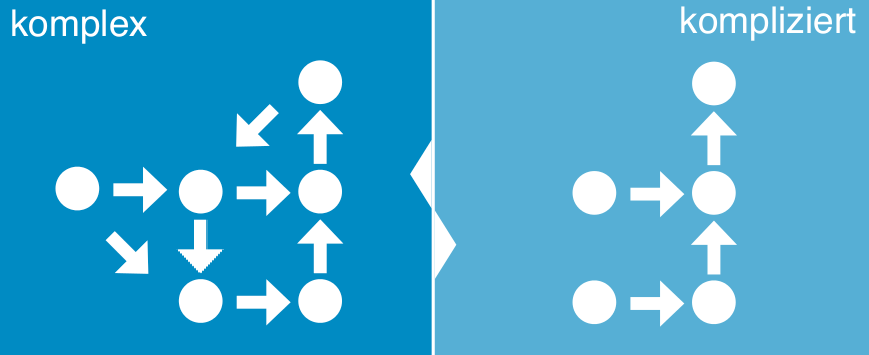
\includegraphics[width=0.6\linewidth]{images/komplex-kompliziert.png}
    \end{minipage}
\subsubsection{Prozess}
Ein Prozess besteht aus einer Folge von Tätigkeiten/Aktivitäten, die aus einer Reihe von Inputs einen oder mehrere bestimmte Output(s) erzeugen.
\subsubsection{Modell}
Ein Modell ist eine Abstraktion eines Systems, welches eine Menge von Annahmen und Näherungen über das Systemverhalten trifft, welche relevant für die Fragestellung sind.
Das Studieren und Experimentieren an einem Modell, anstatt am realen System, hat folgende Vorteile:
\begin{itemize}
    \item schneller, einfacher, billiger, sicherer
    \item Fehler werden am Modell und nicht am realen System gemacht
    \item System kann durch Modellierung(sprozess) besser verstanden werden
\end{itemize}
\subsubsection{Validierung und Verifikation}
\begin{minipage}[t]{1\textwidth}
    \centering
	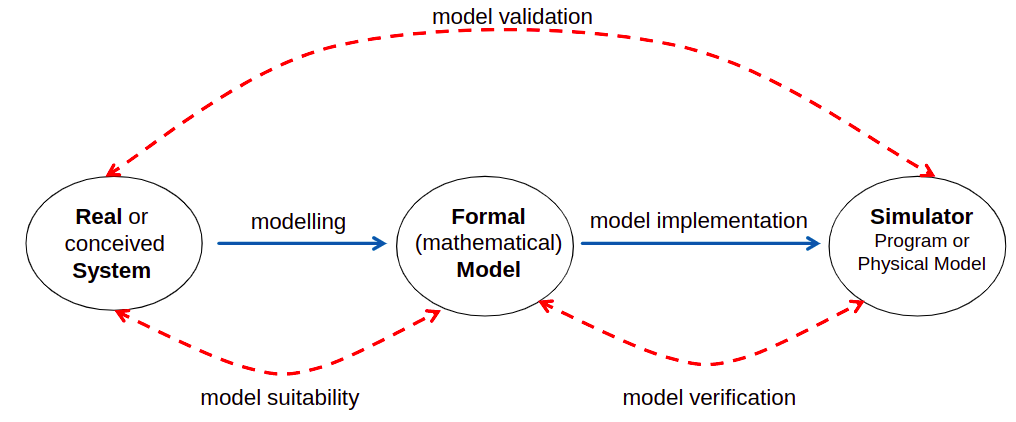
\includegraphics[width=0.9\linewidth]{images/simulationsphasen.png}
\end{minipage}

Mit der \textbf{Verifikation/Verifizierung} oder auch Modell-Korrektheit wird überprüft, ob die Modelldaten korrekt, also gemäss Spezifikation (Pflichtenheft), erfasst sind.

Mit der Modell-Validität oder auch \textbf{Validierung} wird überprüft, ob das Modell gültig hinsichtlich der Anforderungen des Kunden ist.



\subsubsection{Experiment}
Ein Test, eine Untersuchung oder eine Prozedur, um eine Hyptohese zu überprüfen, ein bestimmtes Verhalten aufzudecken oder um eine Entscheidung zu begründen.

\subsection{Verschiedene Simulationsansätze}
\begin{itemize}
    \item FEM (Finite-Elemente-Methode) - Verformung z.B an einem Auto*
    \item MKS (Mehr Körper Simulation) - Untersuchung mehrere (unverformbaren) Körper/Objekte*
    \item CFD (Computational Fluid Dynamics) - Strömungssimulationen*
    \item DES (Discrete Event Simulation) / Diskrete Ereignissimulatioin 
    \begin{itemize}
        \item diskret
        \item ereignisgesteuert
    \end{itemize}
\end{itemize}
*\textit{Für uns nicht interessant}

\subsection{Klassifikation von Simulationen}
\begin{minipage}[t]{1\textwidth}
    \centering
	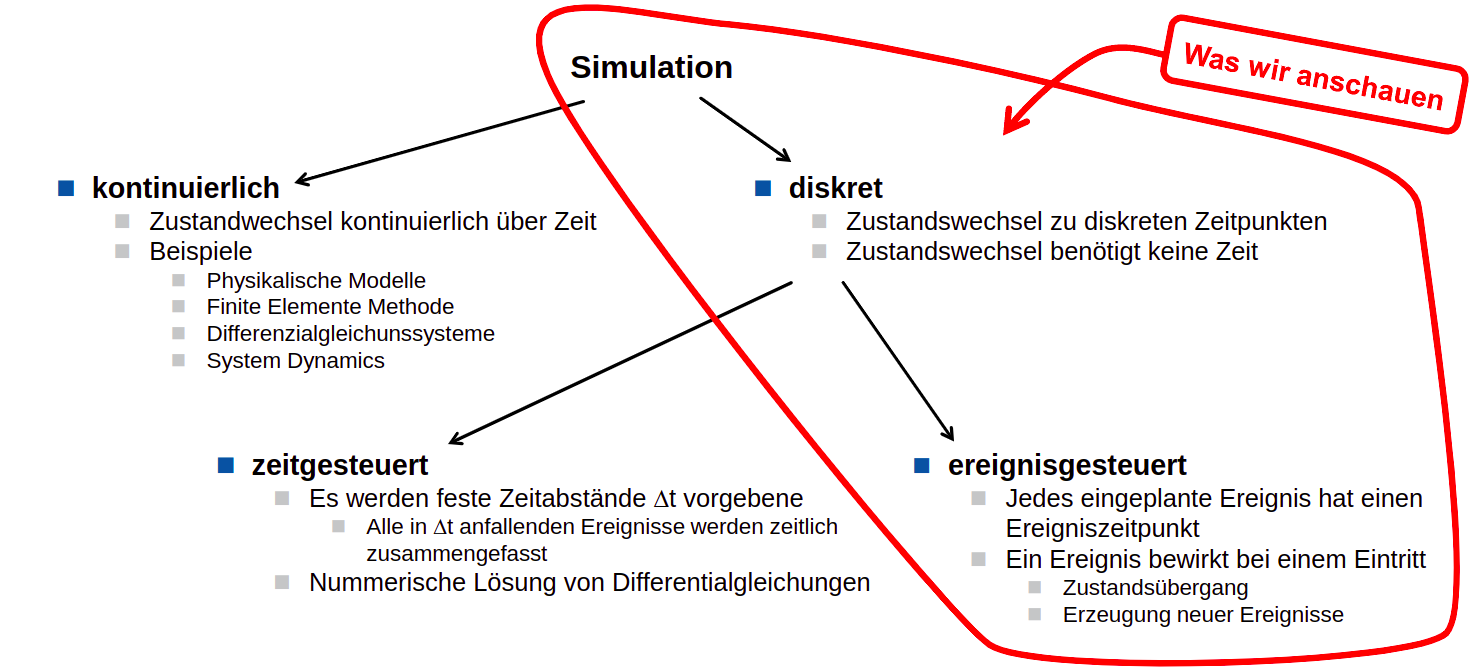
\includegraphics[width=0.9\linewidth]{images/klassifizierung-simulationen.png}
\end{minipage}
\begin{itemize}
    \item Statisch/Dynamisch
    \begin{itemize}
        \item Statisch - Zeit spielt \textbf{keine} Rolle
        \item Dynamisch - Zeit spielt eine wesentliche Rolle
    \end{itemize}
    \item Kontinuierlich/Diskret
    \begin{itemize}
        \item Kontinuierlich - stetiger (ununterbrochener) Zustandswechsel über die Zeit
        \item Diskret - Zustandswechsel zu bestimmten Zeitpunkten
    \end{itemize}
    \item Zeitgesteuert/Ereignisgesteuert
    \begin{itemize}
        \item Zeitgesteuert - Simulation wird fortlaufend in Zeitinkremente eingeteilt und in jedem Zeitintervall Zustandsänderungen untersucht/durchgeführt
        \item Ereignisgesteuert - Zustandsänderungen werden durch eintretende Ereignisse verursacht - Ereigniss hat Eintrittszeitpunkt, jedoch wird simulierte Zeit nicht beachtet
    \end{itemize}
    \item Deterministisch/Stochastisch
    \begin{itemize}
        \item Deterministisch - Werte sind fest bestimmt
        \item Stochastisch - Werte/Ereignisse können zufällig auftreten
    \end{itemize}
\end{itemize}
Die meisten System sind: Dynamisch, Diskret & Stochastisch (SMS konzentriert sich auf solche).
\\

Weitere Infos: \href{https://pdfs.semanticscholar.org/d09e/bff3e7d0145b964fe31cdf31a119a8d7fca7.pdf}{Modellbildung und Simulation}

\subsection{Gründe für ein Simulationsprojekt}
\begin{itemize}
    \item Bestimmung der Variabilität, welche in jedem Prozess vorhanden ist
    \begin{itemize}
        \item unterschiedliche Ergebnisse, welche einen Mittelwert schwanken, wenn man den Wert über die Zeit analysiert 
        \item macht einem das Leben schwer, Simulation kann Abhilfe schaffen
    \end{itemize}
    \item Abbildung eines kompletten Systems 
    \begin{itemize}
        \item ermöglicht Systeminteraktionen/Abhängigkeiten zu studieren
        \item Prozesse werden nicht isoliert angeschaut
        \item kostengünstig \& risikolos
    \end{itemize}
    \item Identifizierung von Engpässen/Bottlenecks, darunter:
    \begin{itemize}
        \item durchschnittliche Wartezeit, die ein Ereigniss auf eine Ressource warten muss
        \item durchschnittliche Anzahl der Ereignisse, die auf eine Ressource warten
    \end{itemize}
    \item Analyse des zeitlichen Verhaltens - Untersuchung und Optimierung der Systemdynamik z.B.
    \begin{itemize}
        \item Mitarbeiterplanung verbessern
        \item Verfügbarkeit und Auslastung von Ressourcen optimieren
        \item Prozessstrukturen und Abläufe besser aufeinander abzustimmen
    \end{itemize}
    \item Animation
    \begin{itemize}
        \item Visualisierung bildet Vertrauen - Kunde sieht seine Prozesse
        \item Wichtig für Validierungs- \& Entscheidungsprozess - \glqq \textit{ die Personen wollen etwas sehen} \grqq
    \end{itemize}
    \item Prozesskomplexität
    \begin{itemize} 
        \item Simulationsprojekte können komplexe Systeme beschreiben/studieren - \glqq \textit{ Nicht so genau wie möglich, sondern so genau wie nötig}\grqq
        \item Komplexität aufteilen - Subsysteme bilden - \glqq \textit{Teile \& Herrsche}\grqq
    \end{itemize}
\end{itemize}

\subsection{Ablauf und Phasen eines Simulationsprojekts}
\begin{minipage}[t]{1\textwidth}
    \centering
	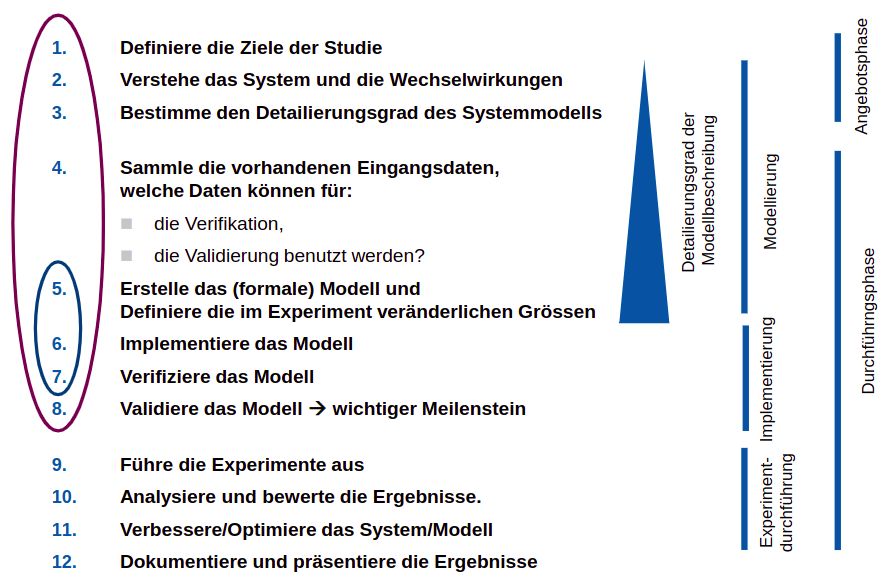
\includegraphics[width=0.9\linewidth]{images/ablauf-simulationsprojekt.png}
\end{minipage}

\subsubsection{Ziele definieren}
Einige Beispiel, wie Ziele in einer Simulationsstudie lauten könnnten:
\begin{itemize}
    \item Lohnt es sich in neue Komponenten zu investieren?
    \item Wo gibt es Bottlenecks und wie kann ich diese reduzieren?
    \item Wie kann ich Resourcen optimal nutzen?
    \item Wie soll ich ein neues System gestalten und wie viele Komponenten brauche ich?
    \item Wie wirkt sich eine konkrekte Systemänderung auf mein Gesamtsystem aus?
    \item Welche Komponenten muss ich wie verändern, um einen besseren Durchsatz zu erreichen?
\end{itemize}

\subsubsection{Modellbildung}
Nachdem das Ziel festgelegt wurde, wird das Modell entwickelt. In diese Phase soll der Prozessablauft beschrieben werden. Es ist wichig festzustellen, wie die Tokens oder Entities durch das System fliessen.
Daher sind gezielte Fragen an die Prozesseigentümer und -teilnehmer zu stellen. 
\begin{itemize}
    \item Wie bewegt sich ein Entity durch das System?
    \item Welche Bedingunen sind im System fomuliert?
    \item Welche Regeln müssen eingehalten werden?
    \item Gibt es irgendwelche Ausnahmen zu den Regeln? 
    \item Welche Bottlenecks sind zurzeit bekannt?
\end{itemize}

\info{Vergleiche Aussagen miteinander}{Da sicherlich nicht alle mit einer Veränderungen einverstanden sind, ist es wichtig, die einzelnen Antworten mit Quervergleichen zu überprüfen. Es wird nicht immer die Wahrheit erzählt.}

\subsubsection{Key Performance Indicators}
In einem Simulationsprojekt ist es wichtig Schlüsselwerte, sogenannte Key Performance Indicators (KPI), zu definieren. Damit man weiss, welche Werte und Ereignisse zu beobachten sind, sollte man sich \glqq \textit{what-if\grqq-Szenarien}  notieren:
\begin{itemize}
    \item Was passiert, wenn wir eine Maschine hinzufügen oder entfernen?
    \item Was passiert, wenn wir die Gabelstaplergeschwindigkeit erhöhen?
    \item Was passiert, wenn wir eine neues Schichtensystem einführen?
\end{itemize}
Diese Fragen sollten zu einem späteren Zeitpunkt mittels Simulationen beantwortet werden können.
\newline
\newline
Einige Beispiele für KPIs sind:
\begin{itemize}
    \item Resource Utilizations 
    \item Totaler Durchsatz
    \item Entities in Progress
    \item Durchlaufzeit
    \item Kosten
    \item Fehlbestand
    \item Wartezeit in einer Queue
    \item Anzahl in einer Queue
\end{itemize}

\subsubsection{Ergebnisse}
Wichtig ist es, mit dem Kunden die zu erwartenden Ergebnisse im Vorhinein zu definieren. Es wird klar definiert, was und in welcher Form abzugeben ist. Bei einer Simulation werden Ergebnisse in der Regel in einer Spezifikation datgestellt. Diese beinhaltet beispielsweise folgende Dinge: 
\begin{itemize}
    \item Simulation Modelverhalten
    \begin{itemize}
        \item Modellstruktur und Entity-Fluss
        \item Logisches Verhalten
        \item Temporales Verhalten 
    \end{itemize}
    \item Simulation inkl. Modelanimation
    \item Dokumentationen
    \item User Interface
    \item Analysereport - detaillierten Report zu allen Szenarieren und Ereignissen inkl. Empfehlungen
    \item Regelungen der Lizenzen
    \item Schulungsunterlagen
    \item Regelung des Kundensupports
\end{itemize}
Sobal man weiss und definiert ist, was der Kunde genau will, kann man anhand der vorhandenen Informationen einen Projektplan erstellen.

\subsection{Zusammenfassend: Formalisierung des IST-Models}
Somit kann man ein IST-Model wie folgt formalisieren:
\begin{itemize}
    \item Fehlende Daten ergänzen
    \item Annahmen treffen
    \item Fragen!
    \item Analyse und Berechnungen soweit möglich
    \item Beobachtungen festhalten
    \item Anforderunfgen an die Implementierung festhalten
\end{itemize}

\section{Modellierung}
\subsection{Vertiefung: Was ist ein Modell?}
Wir haben bereits definiert, dass ein Modell ein vereinfachtes Abbild der Wirklichtkeit ist.
Ebenfalls wird ein Modell durch diese drei Merkamle gekenntzeichnet:
\begin{enumerate}
    \item \textbf{Abbildung} - Braucht eine geeignete Beschreibunugssprache!
    \begin{itemize}
        \item Modell von oder für etwas
        \item nämlich Abbildung/Repräsentation eines Originals
    \end{itemize}
    \item \textbf{Verkürzung} - Braucht eine genaue Definition der Ziele/Beobachtungen
    \begin{itemize}
        \item Ein Modell erfasst nur relevante Attribute des Originals
    \end{itemize}
      \item \textbf{Pragmatismus} - Braucht eine angepasste Modellierungsmethode
    \begin{itemize}
        \item Ein Modell ist seinem Original nicht eindeutig zuzuordnen
        \item Sie erfüllen nur Ersetzungsfunktionen
        \begin{itemize}
            \item \textit{für wen?} - für bestimmte Subjekte(= wer handelt) 
            \item \textit{wann?} - innerhalb bestimmter Zeitintervalle
            \item \textit{wozu?} - unter Einschräkungen auf bestimmte gedankliche oder tatsächliche Operationen
        \end{itemize}
    \end{itemize}
\end{enumerate}

Zusätzlich gilt für jedes Modell:
\begin{itemize}
    \item besteht aus einer Menge von Objekten (Individuen) und Attributen
    \item Objekte (Individuen) sind individuell erkennbar und von anderen Objekten eindeutig abgrenzbar
    \item Attribute beschrieben Objekte oder wiederrum andere Attribute
\end{itemize}
Es passt also ganz gut zu einem objektorientierten Ansatz.

\subsection{Modellierung}
Modellierung ist der Prozess der Abbildung der reduzierten Realität in ein geeignetes Modell.
Wir erstellen dabei abstrakte, durch eine Sprache ausgedruckte, Modelle. Dabei ist eine Sprache definiert
durch eine strukturierte Menge von Zeichen. In der Regeln sind Beschreibungssprachen gekenntzeichnet, durch eine formale Syntaxt, eine formale Semantik. Somit sind diese Sprachen alle formale Sprachen.
\newline


Grundsätzlich sind folgende Punkte festzulegen:
\begin{itemize}
    \item Verwendete Notation
    \item Gemeinsamer Zeichenvorrat
    \item Regeln für die Bildung von Zeichenstrukturen (Syntax)
    \item Bedeutung der Zeichen, d.h der ihnen zugeordneten begrifflichen Vorstellung (Semantik)
\end{itemize}
Damit  alle vom Gleichen sprechen, müssen Bedeutungsdefinitonen (Ontologien\footnote{Ontologien sind formale Modelle einer Anwendungsdomäne, die dazu dienen, den Austausch und das Teilen von Wissen zu erleichtern. Damit Menschen über ein Modell kommunizieren können, benötigen sie eine gemeinsame Ontologie des Anwendungs- und Wissensbereichs, der dem Modell zu Grunde liegt 
}) erstellt werden. Bei der diskreten Ereignis-Simulation müssen folgende Elemente klar definiert sein:
\begin{itemize}
    \item Architektur bzw. Systemstruktur 
    \item Ereignis
    \item Prozessmodell
    \item Prozesslogik
    \item Ressoruces 
    \item Entity
\end{itemize}

\subsection{Arbeitsphasen der Modellierung}
\begin{enumerate}
    \item Herstellung der Technischen Klarheiten (Big Picture)
    \item Datenbeschaffung
    \item Durchführung der Modellbildung 
    \item Experimentenplanung
    \item Verifikation und Validierung
    \item Dokumentation und Präsentation
    
\end{enumerate}
\subsection{Event Storming}
\subsubsection{Grundlagen}
Bevor eine weitere Modellspezifikation in Angriff genommen wird, sollte mit Event Storming ein Überblick über das System und dessen relevanten Prozesse und Entscheidungen gewonnen werden. Bei diesem Vorgehen orientiert man sich an den verschiedenen Ereignissen (Domain-Events), die während eines Arbeitsablaufes (Work-Flows) geschehen.
\subsubsection{Ziel}
Dabei soll schlussendlich folgende Ziele erreicht werden:
\begin{itemize}
    \item Den benötigten Detaillierungsgrad bestimmen
    \item die Prozesschritte festlegen
    \item die Ressourcen definieren
    \item die Entscheidungspunkte im System identifizieren
\end{itemize}
\subsubsection{Elemente}
\begin{itemize}
    \item \textbf{(Domain-)Events} sind Ereignisse, die zu einem spezifischen Zeitpunkt geschehen und dann zur Historie des System gehören. Daher werden diese auch in der Vergangenheitsform beschrieben. Diese werden in \colorbox{orange}{orange} notiert und in chronologischer Reihenfolge angebracht.
    
\begin{minipage}[t]{1\textwidth}
    \centering
	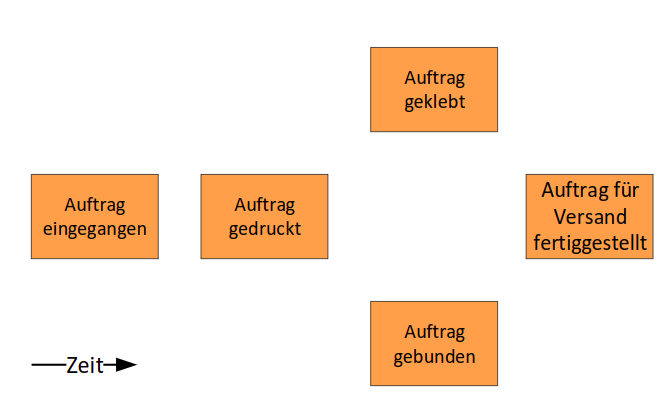
\includegraphics[width=0.6\linewidth]{images/domain-events.png}
\end{minipage}

\info{Prozess}{Hinter Domain-Events steht oft ein Prozess, der mit diesem Ereignis abgeschlossen wurde.}
 
\end{itemize}

\item \textbf{Ressourcen} werden verwendet, um die Durchführung eines Prozesses zu ermöglichen. Ressourcen sind beispielsweise Arbeitsplätze, Mitarbeiter, Maschinen oder Verbrauchtsmaterial. Ressourcen werden dabei \colorbox{blue}{\color{white}blau} dargestellt, und bei den Domain-Events, wo sie gebraucht werden, platziert.



\begin{minipage}[t]{1\textwidth}
    \centering
	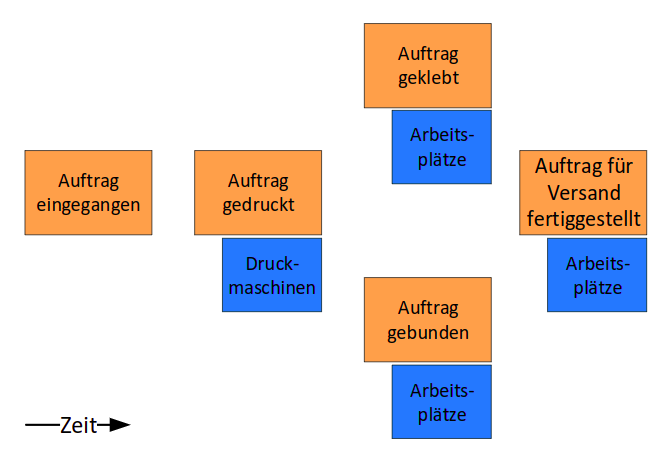
\includegraphics[width=0.6\linewidth]{images/ressourcen.png}
\end{minipage}

\info{Mehrfachverwendungen}{Wird eine Ressource bei mehreren Domain-Events verwendet, so muss dies gekenntzeichnet werden. Dafür eignet sich einen roten Punkt und eine ID.}


\item \textbf{Daten} spezifizieren die Ressourcen und die Prozesse, die auf den jeweiligen Domain-Events ablaufen, näher. Beispiele dafür sind:
\begin{itemize}
    \item Informationen zu Kapazitäten von Ressorucen oder Pufferplätzen
    \item Prozess-, Umrüst- und Reininungszeiten
    \item Ausfallzeiten und Wartungsinformationen
    \item Schichtpläne und viel mehr
\end{itemize}
Diese werden mit einem \colorbox{green}{grünen} Colorcode notiert und unter den jeweiligen Ressourcen platziert.

\begin{minipage}[t]{1\textwidth}
    \centering
	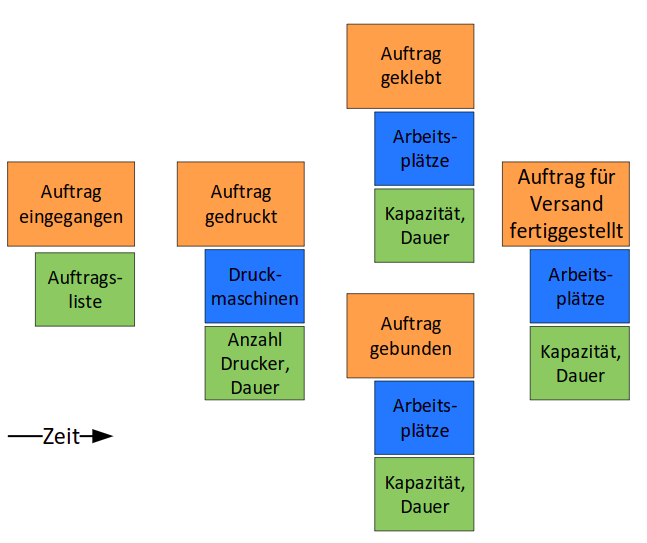
\includegraphics[width=0.6\linewidth]{images/daten.png}
\end{minipage}

\item \textbf{Logik} wird wie gewohnt mit Pfeilen und Gateways gezeichnet. Dabei stellt ein Pfeil einen Übergang und ein Gateway eine Verzweigung respektiv ein Zusammenführung dar. Werden bei einem Domain-Ereignis komplexere Verhalten ausgelöst, so muss dies mit \colorbox{yellow}{gelb}  markiert und beim jeweiligen Event platziert werden. 
    
\begin{minipage}[t]{1\textwidth}
    \centering
	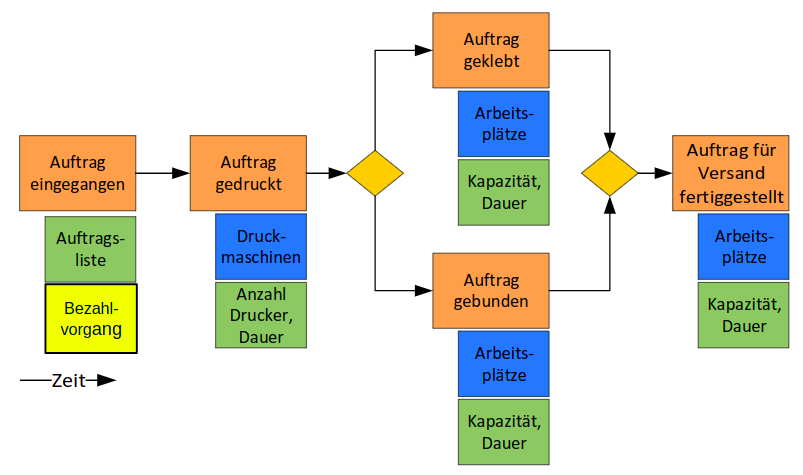
\includegraphics[width=0.6\linewidth]{images/logik.png}
\end{minipage}

\subsection{BPMN}
\subsubsection{Grundlagen}
BPMN bedeutet Business Process Model and Notation und ist eine Flow Chart oder Token und Event basierte Beschreibungssprache. Sie erlaubt die Beschreibung (nebenläufiger) Prozesse/Systeme.
Ebenfalls unterstützt es weitere Sprachkonzepte aus dem objektorientierten Umfeld (SysML, UML). Dies hat der Vorteil, dass die Spezifikation verfeinert werden kann. Zusätzlich ist es möglich, Informationen zu Modellkomponenten zu geben, welche die Simulation der Prozesse ermöglichen (beispielsweise Input Buffer). 

\subsubsection{Übersicht Diagrammelemente}
\begin{minipage}[t]{1\textwidth}
    \centering
	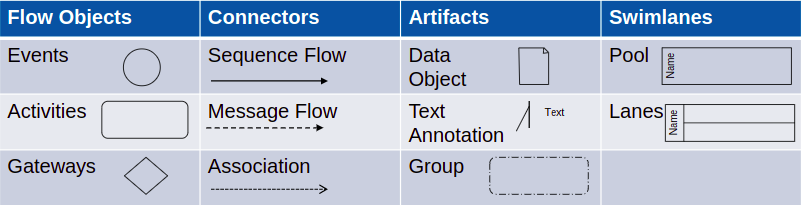
\includegraphics[width=0.8\linewidth]{images/BPMN_diagrammelemente.png}
\end{minipage}

\subsubsection{Prozess}
Beim Prozess unterscheidet man zwischen \textit{Task} und \textit{Sub-Process}.
\begin{itemize}
    \item \textbf{Ein Task} ist ein atomarer Prozess. Das bedeutet er kann/wird nicht weiter unterteilt.
    \item  \textbf{Ein Sub-Process} ist ein Prozess, welcher weiter unterteilt ist. 
    \begin{itemize}
        \item besteht aus weiteren Tasks und/oder Sub-Prozessen.
        \item wird benötigt, um eine verschachtelte (nested) Struktur zu beschreiben.
    \end{itemize}
\end{itemize}

\begin{minipage}[t]{1\textwidth}
    \centering
	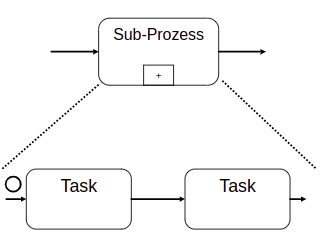
\includegraphics[width=0.4\linewidth]{images/BPMN_process.png}
\end{minipage}

\subsubsection{Token}
Ein Token ist ein Objekt, welches \textbf{durch den Prozess fliesst}. Es ist möglich, dass beim Durchlauf Token erzeugt, verzögert oder zerstört werden. Ebenfalls besitzt ein Token Attribute. Diese können durch einen Prozess verändert werden und bestimmen, wie mit dem Token innerhalb des Prozesses verfahren wird.

\begin{minipage}[t]{1\textwidth}
    \centering
	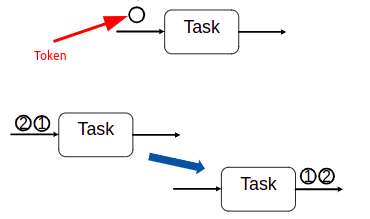
\includegraphics[width=0.4\linewidth]{images/BPMN_token.png}
\end{minipage}
\info{Überholen}{Gleichzeitig bearbeitete Token können sich überholen. Siehe Reihenfolge Token 1 \& 2 im unteren Bildteil.}

\subsubsection{Ressourcen}
Um ein Task oder ein Sub-Prozess auszuführen, braucht dieser Zeit (Bearbeitungszeit), welche man im BPMN Ressourcen nennt.

Die Bearbeitungszeit kann durch einen \textbf{Interrupt} unterbrochen werden, um die Ressource einen höher priorisierten Prozess zur Verfügung zu stellen.

Grunfsätzlich unterscheidet man zwischen zwei verschiedenen Situationen:
\begin{enumerate}
    \item Die Anzahl der Ressourcen ist begrenzt
    \begin{itemize}
        \item Eventuell können nicht alle eintretenden Token gleichzeitig bearbeitet werden
        \item Nicht bearbeitete Token können gespeichert, verworfen oder blockiert werden
    \end{itemize}
    \item Die Anzahl der Ressourcen ist unbegrenzt
    \begin{itemize}
        \item Es können alle eintretenden Token gleichzeitig bearbeitet werden
        \item so stellt der Prozess nur eine Verzögerung (Delay) dar
    \end{itemize}
\end{enumerate}

\subsubsection{Events}
Ein Event ist etwas, welcher zu einem bestimmten Zeitpunkt im Modell passiert. Ein Event beeinflusst den Ablauf eines Prozesses. Es besteht aus einem Start- und einem Endpunkt.
Wir unterscheiden zwischen 
\begin{itemize}
    \item Start-Event - einfacher, dünner Rand
    \begin{itemize}
        \item Markiert, wo ein Prozess startet
        \item erzeugt einen Token
        \item Differzierung durch verschiedene Symbole
        \begin{itemize}
            \item None: Start von Sub-Prozess oder wenn Start nicht definiert
            \item Message: Eintreffen einer Nachricht
            \item Timer: Definition von Ablauf: einmalig, periodisch
            \item Condition/Rule: Eintreffen von bestimmter Bedingung 
            \item Signal: Erhalten eines bestimmten Signals
        \end{itemize}
    \end{itemize}
    \item Intermediate-Event - doppelter Rand
    \begin{itemize}
        \item Treten auf, wenn Prozess bereits gestartet wurde
        \item Tigger/Auslöser sind durch Piktogramme definiert - es können weitere definiert werden
        \item Platzierung:
        \begin{itemize}
            \item Zwischen Prozessen
            \item An die Grenze eines Prozesses
        \end{itemize}
    \end{itemize}
    \item End-Events - dicker Rand
    \begin{itemize}
        \item Zeigen wo Prozesse terminieren
        \item Dabei werden Token vernichtet
        \item Können wieder Events auslösen
    \end{itemize}
\end{itemize}
    \begin{minipage}[t]{0.3\textwidth}
    \centering
    \textbf{Start-Events}
    \newline
	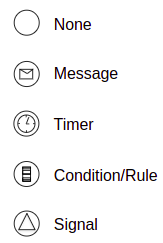
\includegraphics[width=0.65\linewidth]{images/BPMN_start-event.png}
    \end{minipage}
    \begin{minipage}[t]{0.3\textwidth}
    \centering
    \textbf{Intermediate-Events}
    \newline
	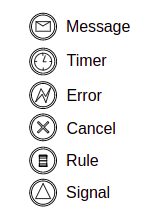
\includegraphics[width=0.625\linewidth]{images/BPMN_intermediate-events.png}
    \end{minipage}
    \begin{minipage}[t]{0.3\textwidth}
    \centering
    \textbf{End-Events}
    \newline
	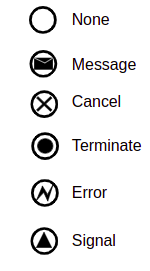
\includegraphics[width=0.55\linewidth]{images/BPMN_end-events.png}
    \end{minipage}
\subsubsection{Gateways}
Gateway erlauben es den Fluss von Token zu steuern und zu kontrollieren. Verschiedene Gateway-Typen werden durch verschiedenen interne Marker definiert. Gatewys teilen oder vereinigen den Fluss von Token - es muss der gleiche Gateway-Typ bei der Teilung und der Verzweigung verwendet werden.
Wir unterscheiden zwischen folgenden verschiedenen Gateways:\\


\begin{minipage}[t]{1\textwidth}
    \centering
	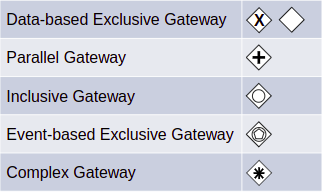
\includegraphics[width=0.6\linewidth]{images/BPMN_gateways-overview.png}
\end{minipage}


\begin{itemize}
    \item Exclusive Gateway
    \begin{itemize}
        \item Übergruppe von XOR-Gateways, um den Fluss zu steuern
        \item Entscheidungen können: Datenbasiert, zufällig oder an Bedingungen geknüpft sein
    \end{itemize}
    \item Data-based Gateways
    \begin{itemize}
        \item Pfad anhand Bedingungen gewählt z.B
        \begin{itemize}
            \item Systemzustand
            \item Zustand des eintreffenden Tokens
            \item Gewichtung des Pfades
        \end{itemize}
        \item Trifft keine Bedingung zu: Default-Path oder Warteschlange (bis eine Bedingung erfüllt)
    \end{itemize}
    \item Parallel Gateways
    \begin{itemize}
        \item Prozess teilt sich auf (Token geklont) und Tasks parallel ausgeführt
        \item Beim Zusammenführen müssen alle parallelen Pfade fertig sein (sonst blockiert)
    \end{itemize}
    \item Inclusive Gateways
    \begin{itemize}
        \item Token wird vervielfacht und läuft parallel weiter
        \item Mehrere oder alle Möglichkeiten möglich
        \item Im Gegensatz zum Parallel GW, mehr als zwei parallele Tasks möglich
    \end{itemize}
    \item Event-based Gateway
    \begin{itemize}
        \item Wegauswahl hängt vom geworfenen Events ab, z.B.
        \begin{itemize}
            \item Eintreffen einer Nachricht
            \item Einreffen eines Signales
            \item Ablauf eines Timers
        \end{itemize}
        \item Eintreffende Token müssen gegebenenfalls im Gateway zwischengespeichert werden (bis Event ausgeführt wird)
        \item Event löst Folgeprozess aus
    \end{itemize}
    \item Coplex Gateway - Frei zu definieren, wenn möglich nicht verwenden
\end{itemize}

   \begin{minipage}[t]{0.3\textwidth}
    \centering
    \textbf{Exclusive Gateway}
    \newline
    \newline
    \newline
    \newline
    \newline
	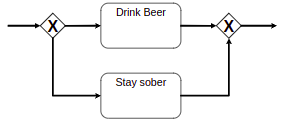
\includegraphics[width=1.05\linewidth]{images/BPMN_exclusive-gateway.png}
    \end{minipage}
    \begin{minipage}[t]{0.3\textwidth}
    \centering
    \textbf{Data-based Exclusive Gateway}
    \newline
    \newline
	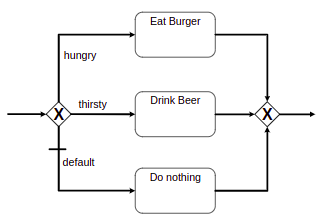
\includegraphics[width=1.025\linewidth]{images/BPMN_data-based-exclusive-gateway.png}
	\newline
    \end{minipage}
    \begin{minipage}[t]{0.3\textwidth}
    \centering
    \textbf{Parallel Gateway}
    \newline
    \newline
    \newline
    \newline
    \newline
	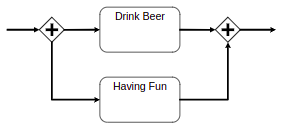
\includegraphics[width=1.05\linewidth]{images/BPMN_parallel-gateway.png}
    \end{minipage}
    
    \begin{minipage}[t]{0.3\textwidth}
    \centering
    \textbf{Inclusive Gateway}
    \newline
	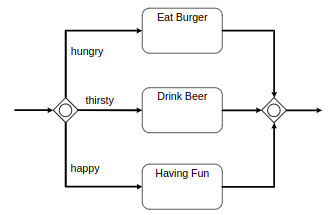
\includegraphics[width=1.05\linewidth]{images/BPMN_inclusive-gateway.png}
    \end{minipage}
    \begin{minipage}[t]{0.3\textwidth}
    \centering
    \textbf{Event-based Gateway}
    \newline
	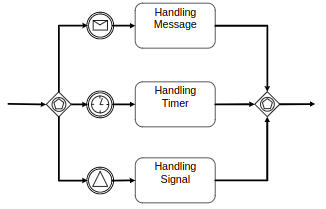
\includegraphics[width=1.05\linewidth]{images/BPMN_event-based-gateway.png}
    \end{minipage}
    \begin{minipage}[t]{0.3\textwidth}
    \centering
    \textbf{Complex Gateway}
    \newline
	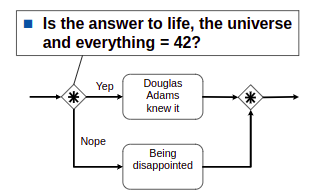
\includegraphics[width=1.05\linewidth]{images/BPMN_complex-gateway.png}
    \end{minipage}
    
\subsubsection{Artefacts}
Im BPMN gibt es auch Artefakte, welche sehr nützlich sein können. Dabei unterscheiden wir zwischen folgenden Untertypen:
\begin{itemize}
    \item \textbf{Annotation} - ein Kommentar, der einem Element eines Prozesses zugeordnet werden kann. 
    \item \textbf{Data Object} - ein Artefakt, das den Geschäftsprozess bearbeitet
    \item \textbf{Group} - ein visuelles Hilfsmittel, um Geschäftsprozesse zusammenzufassen.  
\end{itemize}
\info{Verwechslungsgefahr}{\textbf{Achtung:} eine Group ist nur ein visuelles Hilfsmittel und darf nicht mit einem Sub-Process verwechselt werden.}

\subsection{simBPMN}
simBPMN ist eine Erweiterung für BPMN, welche für Simulationsmodelle gedacht ist. Die verschiedenen Elemente können so klarer aufgezeichnet werden und sind genau definiert.

\subsubsection{Architektur/Struktur vs Prozesslogik}
Unter Entity-Flow vesteht man die Gesamtstruktur des Systems. Die Entities fliessen durch das Gesamtsystem und werden von einigen Prozessen bearbeitet. Aus diesem Grund findet man in der Architektur auch die Begriffe  \textit{Process} und \textit{Entity},

Unter Prozesslogik oder auch Token-Flow versteht man die Logik eines einzelnen Prozesses des Gesamtsystems. Daher findet man in der Prozesslogik auch die Begriffe \textit{Process-Step} und \textit{Token}.

\begin{minipage}[t]{1\textwidth}
    \centering
	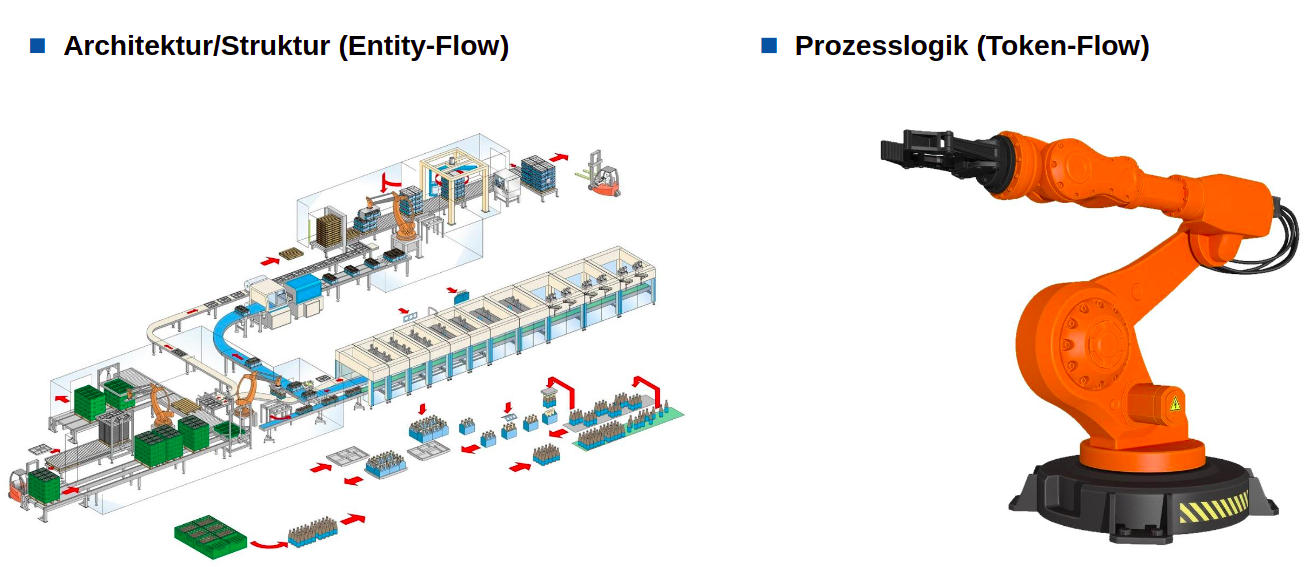
\includegraphics[width=0.8\linewidth]{images/simBPMN_architektur_vs_prozesslogik.png}
\end{minipage}


\subsubsection{Process}
\begin{minipage}[t]{0.7\textwidth}
Ein Process wird \colorbox{red}{rot} gekenntzeichnet und hat folgende Eigenschaften:
\begin{itemize}
    \item Besitzt eine ID
    \item Kann verschiedene Zustände annehmen, diese können sich ändern
    \item Führen Verhaltensvorschrift aus
    \item Verhaltensvorschrit kann geändert werden, ohne den Prozess zu zerstören
    \item Mehrere Prozesse mit der gleichen Verhaltensvorschrift möglich
    \item Benötigt zur Ausführung Ressourcen und Zeit
    \item Besitzt Prozesseingang mit Eingangspuffer
    \item Besiztz Proessausgang mit Ausgangspuffer
    \item Kann Eingangs- in Ausgangselement transformieren oder Elemente zerstören
    \item Kann Ausgangselemente spontan erzeugen
\end{itemize}
\end{minipage}
\begin{minipage}[t]{0.2\textwidth}
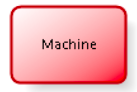
\includegraphics[width=0.6\linewidth]{images/simBPMN_process.png}
\end{minipage}

\subsubsection{Entity}
\begin{minipage}[t]{0.7\textwidth}
Eine Entitiy wird \colorbox{yellow}{gelb} dargestellt und hat folgende Eigenschaften:
\begin{itemize}
    \item Besitzt einen Zustand
    \item Besitzt Attribute
    \item Wird von Prozess zu Prozess weitergeleitet
\end{itemize}
\end{minipage}
\begin{minipage}[t]{0.2\textwidth}
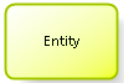
\includegraphics[width=0.6\linewidth]{images/simBPMN_entity.png}
\end{minipage}


\subsubsection{Process-Step}
\begin{minipage}[t]{0.7\textwidth}
Ein Process-Step wird weiss gekenntzeichnet und wie folgt definiert:
\begin{itemize}
    \item Die Abarbeitung einer Serie von Steps wird durch den Ablauf von Token gesteuert
    \begin{itemize}
        \item Ein Token wird ausgelöst durch ein Event
        \item Ein Event wird i.d.R bei einer Zustandsänderung einer Entity oder eines Objektes ausgelöst
    \end{itemize}
    \item Ein Token ist mit dem auslösenden Entity assoziiert - über den Token können auf die Attribute der entsprechenden Entity zugegriffen werden
\end{itemize}
\end{minipage}
\begin{minipage}[t]{0.2\textwidth}
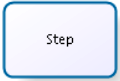
\includegraphics[width=0.6\linewidth]{images/simBPMN_process-step.png}
\end{minipage}

\subsubsection{Token}
\begin{minipage}[t]{0.7\textwidth}
Eine Token wird \colorbox{green}{grün} dargestellt und hat folgende Eigenschaften:
\begin{itemize}
    \item Wird durch ein Event ausgelöst, z.B.
    \begin{itemize}
        \item Entity kommt bei Maschine an
        \item Timmer ist abgelaufen
    \end{itemize}
    \item Besitzt einen Zustand
    \item Kann Zustände ändern
    \begin{itemize}
        \item Eigenen Zustand
        \item Den Zustand des Entity
        \item Den Zustand von Ressourcen
        \item Den Zustand eines anderen Prozesses
        \item Den globalen Zustand
    \end{itemize}
    \item Kann selber Events auslösen
    \item Kann Entities erzeugen oder zerstören
\end{itemize}
\end{minipage}
\begin{minipage}[t]{0.2\textwidth}
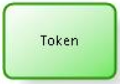
\includegraphics[width=0.6\linewidth]{images/simBPMN_token.png}
\end{minipage}

\subsubsection{Ressourcen}
\begin{minipage}[t]{0.7\textwidth}
Eine Ressource wird \colorbox{brown}{braun} dargestellt und hat folgende Eigenschaften:
\begin{itemize}
    \item Ist mit einem oder mehrere Prozessen assoziiert und wird für dessen Ausführung benötigt. 
    \item Besitzt einen Zustand
    \item Kann Attribute
\end{itemize}
\end{minipage}
\begin{minipage}[t]{0.2\textwidth}
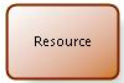
\includegraphics[width=0.6\linewidth]{images/simBPMN_ressource.png}


\end{minipage}

\subsubsection{Überblick}
\begin{minipage}[t]{0.9\textwidth}
\centering
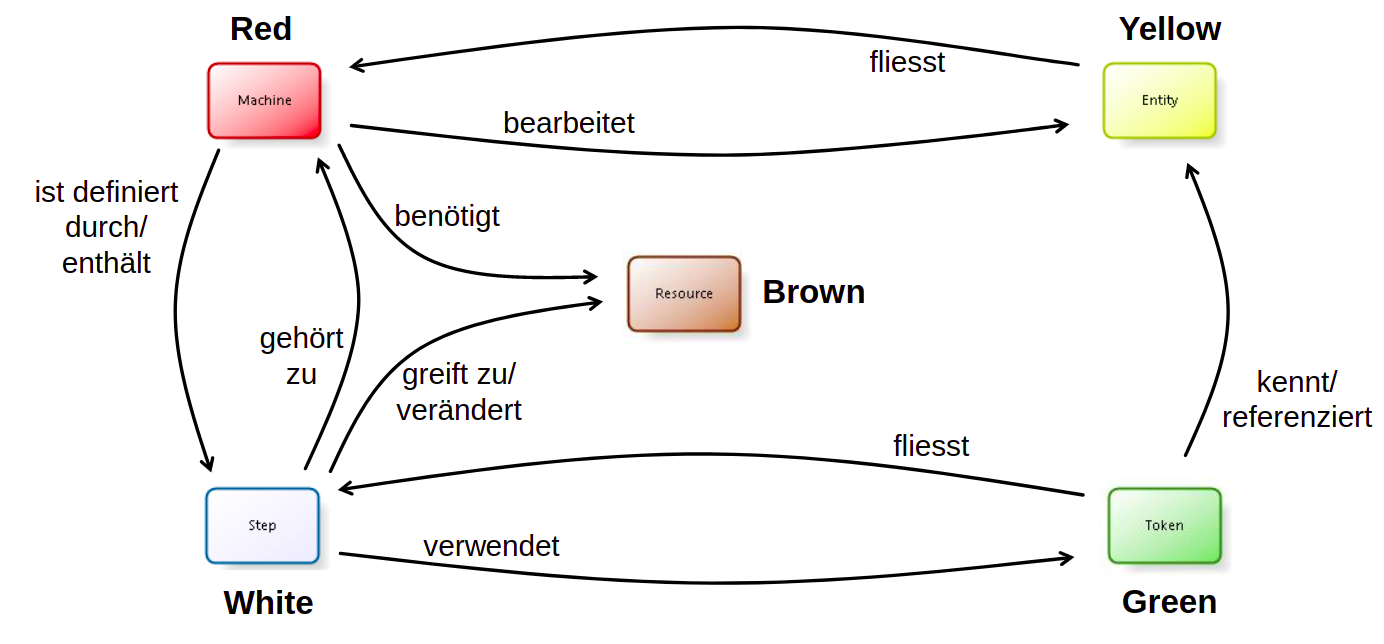
\includegraphics[width=0.9\linewidth]{images/simBPMN_overview.png}
\end{minipage}
\newpage

Nun stellen sich aber mehrere Fragen:
\begin{enumerate}
    \item Wie kann man das Problem der Zusammenführung lösen? - wie weiss man, dass alle parallelen Pfade fertig sind?
    \begin{enumerate}
        \item Man kann Token-Attribute einführen und diese dann überprüfen
    \end{enumerate}
    \item Wie klont man ein Entity? (Entity-Klon Problematik)
    \begin{enumerate}
        \item Nicht alle Entitys sind klonbar (sind ja die Objekte , die durch das Systemfliessen), Token schon, das sind ja «nur» Steuerelement. Ggf. sind Zusatzinformationen den Token, Entitys beizufügen um die Abhängig der Token/Entitys zu beschreiben
    \end{enumerate}
\item Was ist der Unterschied zwischen Token und Entity?
\begin{itemize}
    \item Das Entity ist das Objekt, das durch das System fliesst und beschreibt den möglichen Fow durch das System.
    Zum Beispiel ein Werkstück, das von einer zu einer Arbeitsstation zur nächsten Arbeitsstation weitergereicht wird.
    \item Ein Token beschreibt den logischen Ablauf der Verhaltenslogik, wenn ein bestimmtes Ereignis aufgetreten ist. So kann z.B. das Ereignis, entity an Arbeitsplatz eins angekommen, eine Verhaltenslogik auslösen, wie: Prüfe ob genug Material für die Weiterverarbeitung vorhanden ist, wenn ja .., wenn nein..   
\end{itemize}
\item Was ist das Zusammenspiel von Token, Entity und Event 
\begin{itemize}
    \item Das Event oder Ereignis kann Token oder Entitys auslösen. Token und Entitys können wiederum Ereignisse/Events auslösen. So haben wir die Möglichkeit, einfach konkurrierendes Verhalten(Prozesse, Tasks) zu beschreiben.
\end{itemize}
\end{enumerate}

\subsection{Modellierung des zeitliches Verhaltens mit Warteschlangen}
\subsubsection{Grundlagen}
In den vorherigen Kapitel zum Thema wurde die Zeit ausser Acht gelassen. Jedoch braucht jede Ereignisverarbeitung Zeit und Ressourcen. Durch den unterschiedlichen Zeitbedarf der Ereignisbearbeitung können sich folende Situationen bilden:
\begin{itemize}
    \item Ereignisse können sich überholen (Races)
    \begin{itemize}
        \item Das kann ggf. zu unterschiedlichen logischen Systemverhalten führen
    \end{itemize}
    \item Es stehen nicht genügend Ressourcen zur Ereignisbearbeitung zur Verfügung.
    \begin{itemize}
        \item Somit können sich Ereignisse in einem beliebig grossen Wartebreich stauen (reines Wartesystem)
        \item Stauen sich Ereignisse in einem begrenzen Wartebereich, überschüssige Ereignisse gehen verloren (Warte- Verlustsystem)
        \item Somit können Ereignisse verloren gehen, wenn keine Pufferung vorhanden ist (reines Verlustsystem)
    \end{itemize}
\end{itemize}

\subsubsection{Fragestellung}
In diesem Kapitel interessieren uns vor allem Fragen wie:
\begin{itemize}
    \item \textbf{Ankunftsprozess}
    \begin{itemize}
        \item Wie viele Ereignisse kommen im Mittel pro Zeiteinheit an?
        \item Welcher Verteilungsfunktion folgt der Ereignisstrom?
    \end{itemize}
    \item \textbf{Wie gross ist:}
    \begin{itemize}
        \item die mittlere Aufenthaltsdauer im System?
        \item die Warteschlange?
        \item die mittlere Wartezeit?
        \item die Wahrscheinlichkeit?
        \item die Verlustwahrscheinlichkeit?
        \item die Blockierungswahrscheinlichkeit?
    \end{itemize}
        \item \textbf{Serviceprozess}
    \begin{itemize}
        \item Wie lange dauert die mittlere Servicezeit?
        \item Welche Verteilungsfunktion folgt die Servicezeit?
        \item Wie viele Ressourcen stehen zur Verfügung?
        \item Wie gross ist die Auslastung der Ressourcen?
    \end{itemize}
\end{itemize}

\subsubsection{M/M/1 Queue}

\begin{minipage}[t]{0.9\textwidth}
\centering
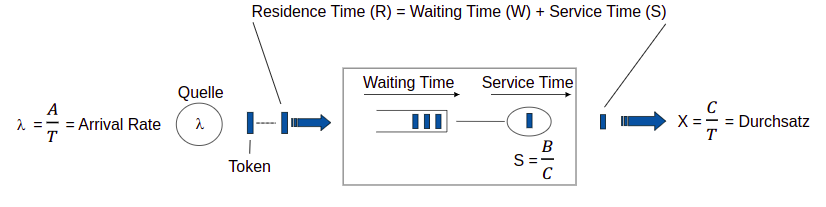
\includegraphics[width=0.9\linewidth]{images/m_m_1-queue.png}
\end{minipage}

Die M/M/1/\infty/$\infty$/FIFO wird auch M/M/1 Queue genannt. Es gelten folgende Eigenschaften:



\begin{itemize}
    \item Es gehen keine Token verloren
    \item Es werden keine neuen Token erzeugt
    \item Es sind alle Werte Mittelwerte
    \item Der Eingangswartebuffer unendlich gross
    \item Der Zeichenvorat der Quelle unendlich gross
    \item Die Bedienungsstrategie ist First In First Out (FIFO) 
\end{itemize}

\textbf{Berechnungen}
\begin{flalign*}
    \begin{aligned}
        A: && \text{Anzahl der ankommenden Token} \\
        T: && \text{Beobachtungszeit des Systems} \\
        C: && \text{Anzahl der abgefertigten Token} \\
        B: && \text{aktive Systemzeit (busy time)} \\
        T: && \text{Beobachtungszeit des Systems} \\
        U: && \text{Utilization } \frac{B}{T}\\
    \end{aligned}
\end{flalign*}
\textit{Arrival Rate:\quad} 
\begin{flalign*}
          \lambda = \frac{A}{T} 
\end{flalign*}
\textit{Service Time:\quad} 
\begin{flalign*}
         S = \frac{B}{C} 
\end{flalign*}
\textit{Durchsatz:\quad} 
\begin{flalign*}
         X = \frac{C}{T} \\
\end{flalign*}
\textit{Residence Time:\quad} 
\begin{flalign*}
R = \textit{Waiting Time (W) + Service Time (S)} \\
\end{flalign*}
\textit{Number in System:\quad} 
\begin{flalign*}
          N = \lambda \cdot R 
\end{flalign*}
\textit{Number in Queue:\quad} 
\begin{flalign*}
        N_Q = \lambda \cdot W 
\end{flalign*}
\textit{Für ein stabiles System gilt:} \\
\begin{flalign*}
	S = \frac{B}{C} \text{ und } 	\lambda = X \Longleftrightarrow \frac{A}{T} = \frac{C}{T} 
\end{flalign*}
\begin{flalign*}
	 \Longrightarrow U = \frac{B}{T} \Longleftrightarrow \frac{B}{C} \cdot \frac{C}{T} 
\end{flalign*}
\begin{flalign*}
	 \Longleftrightarrow S \cdot X  \Longleftrightarrow S \cdot \lambda
\end{flalign*}
\textit{Ferner gilt (im stabilen System):\quad} 
\begin{flalign*}
	\lambda = X \Longrightarrow N = X \cdot R 
\end{flalign*}
\textit{Somit ergibt sich:\quad} 
\begin{flalign*}
	N = \lambda \cdot R \Longrightarrow N = \lambda \cdot (W + S) \Longrightarrow 
\end{flalign*}
\begin{flalign*}
	\Longrightarrow  N = \lambda \cdot W + \lambda \cdot S \Longrightarrow N = N_Q + \lambda \cdot S \Longrightarrow 
\end{flalign*}
\begin{flalign*}
	\Longrightarrow N = N_Q + U 	\Longrightarrow \textbf{U < 1} \Longrightarrow \textbf{stabiles System}
\end{flalign*}
\textit{R in Abhängigkeit von S: } 
\begin{flalign*}
R =  S + W \text{  \quad\quad\quad| } W = N * S
\end{flalign*}
\begin{flalign*}
R = S + N * S  \text{ \quad\quad| } N = \lambda * R
\end{flalign*}
\begin{flalign*}
R = S + \lambda R \cdot S  \text{\quad\quad| Ausklammern}  
\end{flalign*}
\begin{flalign*}
R - \lambda R \cdot S = S
\end{flalign*}
\begin{flalign*}
R \cdot (1 - \lambda S) = S
\end{flalign*}
\begin{flalign*}
    R =  \frac{S}{1 - \lambda \cdot S}
\end{flalign*}
\textit{Zusammenfassend}
\begin{flalign*}
R = S + S(\lambda \cdot R) \text{\quad| }\lambda R = N_Q 
\end{flalign*}
\begin{flalign*}
R =  \frac{S}{(1 - \lambda \cdot S)} \text{\quad\quad| } \cdot \lambda 
\end{flalign*}
\begin{flalign*}
N_Q = \frac{U}{1-U} \text{\quad\quad\quad| } \cdot S 
\end{flalign*}
\begin{flalign*}
W = \frac{S \cdot U}{1-U} 
\end{flalign*}
\begin{flalign*}
U = \frac{B}{C} \cdot \frac{C}{T}
\end{flalign*}
\begin{flalign*}
U = S \cdot \lambda
\end{flalign*}


\subsubsection{Twin Center}

\begin{minipage}[t]{0.9\textwidth}
\centering
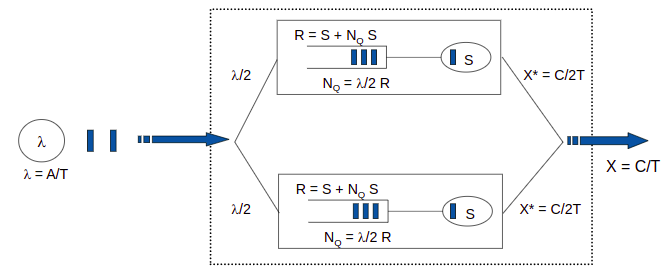
\includegraphics[width=0.9\linewidth]{images/twin-center.png}
\end{minipage}

Beim Twin Center werden zwei M/M/1 Queues parallelgeschalten. So wird die Ankunfrsrate und die Waiting Queue durch zwei geteilt.
Daraus ergibt sich folgendes:
\newline

\textbf{Berechnungen}
\begin{flalign*}
    R = S + S \cdot \frac{N_Q}{2} \text{\quad\quad  | } N_Q = \lambda \cdot R 
\end{flalign*}
\begin{flalign*}
    R =  \frac{S}{1 - \frac{U}{2}} \text{\quad\quad\quad\quad | } \cdot \lambda 
\end{flalign*}
\begin{flalign*}
    N_Q = \frac{\frac{U}{2}}{1-\frac{U}{2}} \text{\quad\quad\quad\quad | } \rho = \frac{U}{2}
\end{flalign*}
\begin{flalign*}
    N_Q = \frac{\rho}{1-\rho}
\end{flalign*}
\begin{flalign*}
\rho = \text{ist die Wahrscheinlichkeit, dass der Server besetzt ist.}
\end{flalign*}
\info{Multi Center}{
Es ist auch möglich, dass mehrere parallele Queues vorhanden sind (Multi Center).
Dann wird der Faktor 2 durch \textit{n} ersetzt.
Somit ergibt sich dann:
\begin{equation*}
    \rho = \frac{U}{n}
\end{equation*}}


\subsubsection{Dual Server}

\begin{minipage}[t]{0.9\textwidth}
\centering
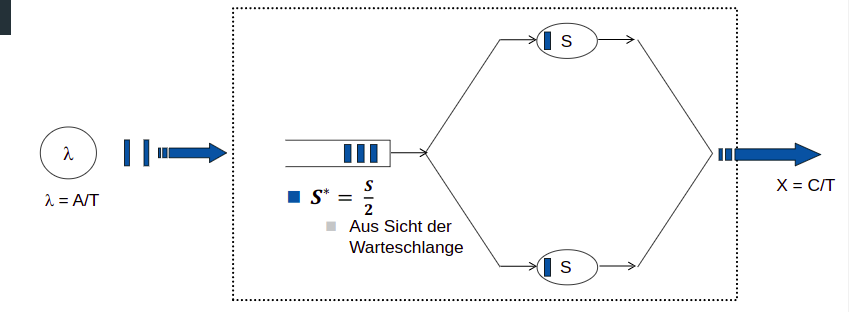
\includegraphics[width=0.9\linewidth]{images/dual-server.png}
\end{minipage}

Beim Dual Server hat man nicht wie beim Twin Center, zwei komplette Warteschlangen, sondern nur eine Queue. Dafür hat man zwei Server.
Somit ergiben sich folgende Eigenschaften:
\newline

\textbf{Berechnungen}
\begin{flalign*}
    S* = \frac{S}{2} \textit{\quad \quad Aus Sicht der Warteschlange} 
\end{flalign*}

\begin{flalign*}
    R = S + S* \cdot \rho N_Q \text{\quad\quad  | } \rho = \frac{U}{2} 
\end{flalign*}
\begin{flalign*}
R = S + \frac{S}{2} \cdot \rho N_Q \text{\quad\quad  | } N_Q = \lambda \cdot R 
\end{flalign*}
\begin{flalign*}
R = S + \frac{S \cdot \lambda}{2} \cdot \rho R \text{\quad\quad  | } \frac{s\lambda}{2} = \frac{U}{2} = \rho 
\end{flalign*}
\begin{flalign*}
   R = S + \rho ^2 R
\end{flalign*}
\begin{flalign*}
   R = \frac{S}{1- \rho ^2} \text{\quad\quad  | } \cdot \lambda 
\end{flalign*}
\begin{flalign*}
   \lambda R = \frac{\lambda S}{1-\rho ^2}
\end{flalign*}
\begin{flalign*}
   N_Q = \frac{2 \rho}{1-\rho ^2}
\end{flalign*}
\info{Multi Server}{Diese Formeln liefern ein exaktes Ergebnis für zwei Server. Bei mehreren ist es eine Näherung. Mehrere Server sind jedoch \textbf{nicht} prüfungsrelevant.}

\subsubsection{Twin Center vs Dual Server}

Bei einem kleinen U ist fast kein Unterschied festzustellen. Bei einer hohen Utilization schneidet der Dual-Server besser ab.


\begin{minipage}[t]{0.9\textwidth}
\centering
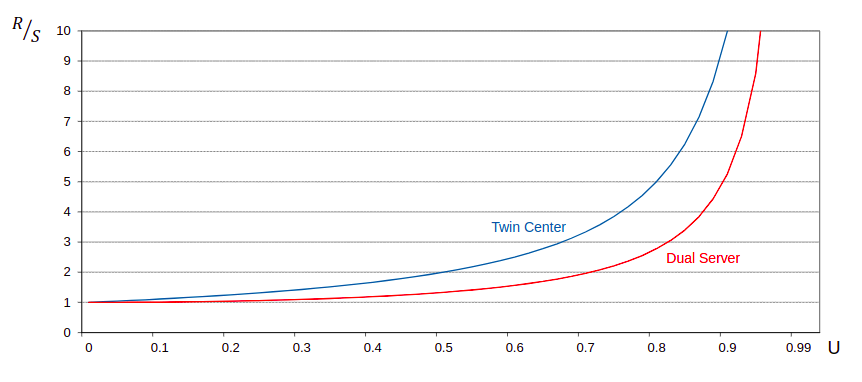
\includegraphics[width=0.9\linewidth]{images/twin-center_vs_dual-server.png}
\end{minipage}

\subsubsection{Feedback Center}

\begin{minipage}[t]{0.9\textwidth}
\centering
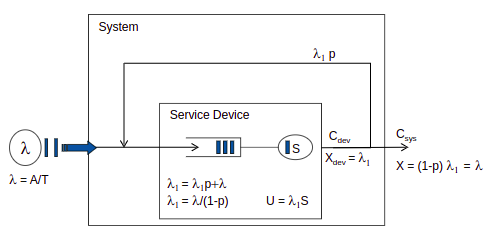
\includegraphics[width=0.9\linewidth]{images/feedback_center.png}
\end{minipage}

Ein Feedback Center arbeit mit Rückkopplung. Daraus ergeben sich folgende Eigenschaften:
\newline

\textbf{Berechnungen}\\
\textit{effektive Ankunftsrate: }
\begin{flalign*}
\lambda _1 = \lambda _1 \cdot \rho + \lambda
\end{flalign*}
\begin{flalign*}
\lambda _1 = \frac{\lambda}{(1 - \rho)}
\end{flalign*}
\begin{flalign*}
U = \lambda _1 \cdot S
\end{flalign*}
\textit{Visits (V) - mittlere Anzahl der Eingaben im Verhältnis zum Ursprungsverkehr:}
\begin{flalign*}
V = \frac{C_d_e_v}{C_s_y_s}
\end{flalign*}
\begin{flalign*}
V = \frac{X_d_e_v}{X}
\end{flalign*}
\begin{flalign*}
V = \frac{1}{1 - \rho}
\end{flalign*}
\textit{Akkumulierte Servicezeit (D) - je grösser die Anzahl der zurückgeleiteten Token sind, desto grösser die akkumulierte Servicezeit:} 
\begin{flalign*}
D = V \cdot S
\end{flalign*}
\begin{flalign*}
R = \frac{D}{1 - \lambda D}
\end{flalign*}


\subsubsection{Closed Queuing Center}

\begin{minipage}[t]{0.9\textwidth}
\centering
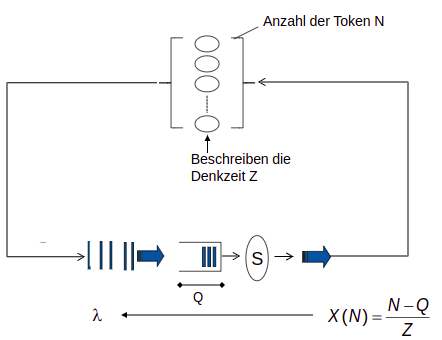
\includegraphics[width=0.9\linewidth]{images/closed-queueing-center.png}
\end{minipage}

Nicht in allen Situationen sind die Anzahl der Token und Ressourcen unbegrenzt. In einem Closed Queuing Center wird daher 
eine Situation mit folgenden Eigenschaften modelliert:
\begin{itemize}
    \item Anzahl der Token ist begrenzt
    \item Sind alle Token in der Queue, so werden keine neuen Token produziert (Lamda gegen 0)
\end{itemize}
\newline

Daraus ergeben sich folgene Formeln:
\newline
\textbf{Berechnungen}
\newline
Anzahl der Token:
\begin{flalign*}
 N
\end{flalign*}
Denkzeit:
\begin{flalign*}
 Z
\end{flalign*}
Abschätzung für m Server:
\begin{flalign*}
\frac{R}{S} = \frac{N}{\rho ^m} - \frac{Z}{S}
\end{flalign*}
Utilisation:
\begin{flalign*}
U = X(N)S = \lambda \cdot S
\end{flalign*}
\textit{Response Time:}
\begin{flalign*}
R = \frac{N}{X(N)} - Z
\end{flalign*}

\section{Nötiges Statistikwissen für dieses Modul}
\subsection{Grundlegende Begriffe der Statistik}
\subsubsection{Zufallsvariable}
Die Zufallsvariable ist die Abbildung, die den Elementen der Ergebnismenge eines Zufallsexperiments reelle Zahlen zuordnet.




\subsubsection{Diskrete Wahrscheinlichkeitsfunktion}

Die \textbf{Diskrete Wahrscheinlichkeitsfunktion ([xi, pi])} weisst einem Element eine Wahrscheinlichkeit zu (diskrete Grösse).
Somit ergeben sich folgende Eigenschaften:
\begin{itemize}
    \item Die Summe aller Einzelwahrscheinlichkeiten ist gleich 1
    \item Die Wahrscheinlichkeit von jedem Ereignis kann abgelesen werden.
\end{itemize}


\begin{minipage}[t]{0.6\textwidth}
\centering
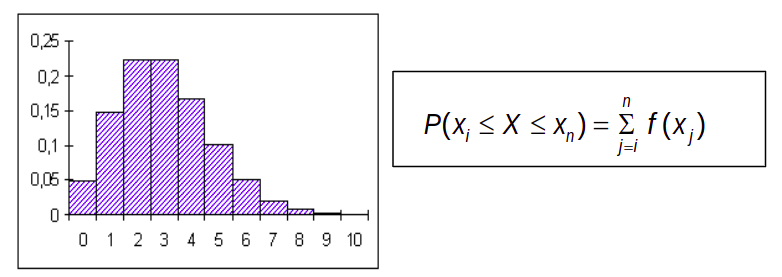
\includegraphics[width=0.9\linewidth]{images/diskrete_wahrscheinlichkeitsfunktion.png}
\end{minipage}
\begin{minipage}[t]{0.325\textwidth}
\centering
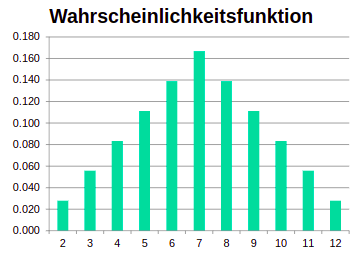
\includegraphics[width=0.9\linewidth]{images/wahrscheinlichkeitsfunktion.png}
\end{minipage}

\subsubsection{Kontinuierliche Verteilungsdichtefunktion }
Die \textbf{Kontinuerliche Wahrscheinlichkeitsdichtefunktion ([(a < x <= b), p])} weisst einem Intervall eine Wahrscheinlichkeit zu.
Da man unendlich viele (kontinuierlich) Werte hat, kann nur die Wahrscheinlichkeit eines Bereiches abgelesen werden.
Somit ergibt sich:
\begin{itemize}
    \item Die Fläche unter der Kurve entspricht der Summe aller Wahrscheinlichkeiten und ist darum = 1. (Integral)
    \item Es kann nur die Wahrscheinlichkeit eines Bereiches (Intervalls) berechnet werde
\end{itemize}

\begin{minipage}[t]{0.55\textwidth}
\centering
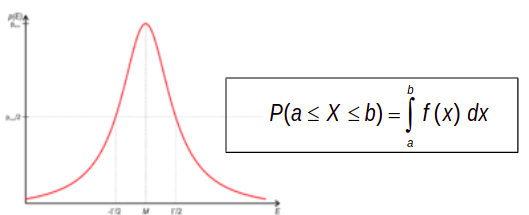
\includegraphics[width=0.9\linewidth]{images/kontinuierliche_verteilungsdichtefunktion.png}
\end{minipage}
\begin{minipage}[t]{0.325\textwidth}
\centering
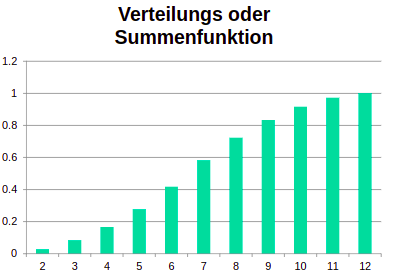
\includegraphics[width=0.9\linewidth]{images/summenfunktion.png}
\end{minipage}

\subsection{Diskrete Verteilungen}
\subsubsection{Bernoulli Prozess}
Als Bernoulli-Prozess wird eine wiederholte Durchführung eines Zufallsvorgangs bezeichnet, wobei gilt: 
\begin{itemize}
    \item Bei jeder Wiederholung interessiert nur, ob ein bestimmtes Ereignis eintritt oder nicht
    \item Die Wiederholungen sind unabhängig
    \item Die Erfolgswahrscheinlichkeit p bleibt gleich
    \item Die Misserfolgswahrscheinlichkeit q ist dann: q = 1 -p
\end{itemize}

\textbf{Berechnungen}
Erwartungswert
\begin{flalign*}
R = \frac{N}{X(N)} - Z
\end{flalign*}
Varianz
\begin{flalign*}
\sigma² = p \cdot q
\end{flalign*}

\subsubsection{Binomial Verteilung}
Die Binomial Verteilung gilt als die wichtigste diskrete Verteilung.
Diese Verteilungsfunktion hat folgende Eigenschaften:
\begin{itemize}
    \item Das Zufallsexperiment unterscheidet nur zwei Ergebnisse (true/false) n=1
    \item Das Experiment wird n-mal wiederholt
    \item Gesucht ist die Wahrscheinlichkeit, dass bei n-maliger Durchdführung ein Ereignis genau, mindestens oder höchstens x-mal eintrifft.
\end{itemize}

\newline
\textbf{Berechnungen}
\textit{Wahrscheinlichkeitsfunktion:}
\begin{flalign*}
f(x) = P(X = x) = \binom{n}{x} p^x(1-p)^n^-^x
\end{flalign*}
\textit{Erwartungswert:}
\begin{flalign*}
E(X) = n \cdot p
\end{flalign*}
\textit{Varianz:}
\begin{flalign*}
Var(X) = np \cdot (1 - p)
\end{flalign*}
\subsubsection{Poisson Verteilung}
Die Poisson Verteilung ist ebenfalls eine wichtige diskrete Verteilung und hat folgende Eigenschaften
\begin{itemize}
    \item Gibt an, wie hoch die Wahrscheinlichkeit ist, dass ein Ereignis (E) in einem Intervall genau oder höchstens eintritt.
    \item Es ist bekannt, dass in dem gegebenen Intervall das Ereignis im Mittel m-mal auftritt
\end{itemize}

\textbf{Anwendung/Beispiele}
\begin{itemize}
    \item Wie hoch ist die Wahrscheinlichkeit, dass: 
    \begin{itemize}
        \item an einem Beobachtungspunkt im Zeitintervall von einer Minute 2 Fahrzeuge vorbeikommen, wenn die durchschnittliche Rate in diesem Intervall bekannt ist
        \item in einer Spinnerei an einem Tag 10 Fadenrisse auftreten
        \item n Ereignisse pro Intervall auftreten
    \end{itemize}
\end{itemize}

\info{Wichtig}{\[
    \mu \text{ gibt eine Rate pro Intervall an und hat grossen Einfluss auf das Aussehen der Verteilung!}
\]}

\textbf{Berechnungen}
\textit{Wahrscheinlichkeitsfunktion:}
\begin{flalign*}
f(x) = P(X = x) = \frac{\mu^x}{x!}e^-^\mu    
\end{flalign*}
\textit{Erwartungswert = Varianz:}
\begin{flalign*}
E(X) = Var(X) = \mu  
\end{flalign*}

\textbf{Hinweise für die Simulation}
\begin{itemize}
    \item In der Simulation wir die Poissonverteilung oft verwendet, um die Rate eines Ankunftsprozesses unabhängiger Entitys zu beschreiben
    \begin{itemize}
        \item Kunden kommen in den einen Laden
        \item Fehler treten auf
    \end{itemize}
    \item Häufig wird auch die \textit{Interarrival Time} benötigt
\end{itemize}
\info{Kehrwert der Rate}{Interarrival Time ist der Kehrwert der Poissonverteilung. Wird viel für die Berechnung benötigt.}

\subsection{Wichtige stetige Verteilungen}
\subsubsection{Rechteck Verteilung}
\begin{minipage}[t]{0.625\textwidth}
\centering
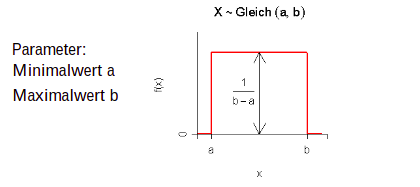
\includegraphics[width=0.9\linewidth]{images/rechteck-verteilung.png}
\end{minipage}

Die Rechteckverteilung hat folgende Eigenschaften:
\begin{itemize}
    \item Eignet sich zur Beschreibung von Vorgängen, bei denen die Ergebnisse nur Zahlen eines gewissen Bereichen ([a,b]) sein können.
    \item Die Wahrscheinlichkeit, dass ein Ergebniss in ein bestimmtes Teilintervall fällt, wurd nur durch desen Länge bestimmt.
    \item Alle Ergebnisse eines bestimmten Intervalls sind gleich wahrscheinlich (gleichverteilt in [a,b])
    \item Oft verwendet als Annahme, wenn keine genaueren Daten vorliegen
\end{itemize}

\textbf{Anwendung/Beispiele}
\begin{itemize}
        \item In einer Stadt verkehren die U-Bahnzügeim Abstand von 10 Minuten. Ziel ist die Ermittlung der Wartezeit eines Fahrgastes, der zu einem zufälligen Zeitpunkt den Bahnsteig betritt. 
        \item Das Drehen eines Glücksrads kann ebenfalls als rechteckverteilte Zufallsvariable beschrieben werden. \\
        Die Auslenkung gegenüber der Ruhelage wird durch eine R(0,2π)-verteilte Größe modelliert. 
\end{itemize}

\textbf{Berechnungen} \\
\\
\textit{Median:}
\begin{flalign*}
E(X) = Median = \frac{a + b }{2}    
\end{flalign*}
\textit{Varianz:}
\begin{flalign*}
Var(X) = \sigma^2  = \frac{1}{12} \cdot (b - a)²    
\end{flalign*}


\subsubsection{Dreieck Verteilung}
\begin{minipage}[t]{0.425\textwidth}
\centering
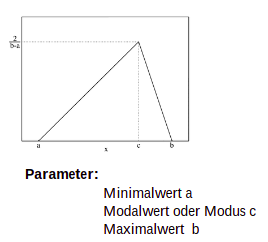
\includegraphics[width=0.9\linewidth]{images/dreieck-verteilung.png}
\end{minipage}
\begin{minipage}[t]{0.45\textwidth}
\centering
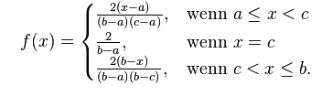
\includegraphics[width=0.9\linewidth]{images/dreieck-definition.png}
\end{minipage}

\textbf{Anwendung/Beispiele}
\begin{itemize}
        \item Zur Beschreibung der Bearbeitungszeit, einer Dienstleistung 
        \begin{itemize}
            \item Bedienzeit an einer Kasse
            \item Zeit eines Produktionsprozesses
            \item Allgemeinen Sericezeiten
            \item einfache Annahmen
        \end{itemize}
\end{itemize}

\textbf{Berechnungen} \\
\\
\textit{Erwartungswert oder Median:}
\begin{flalign*}
E(X) = \frac{a + b + c }{3}    
\end{flalign*}
\textit{Varianz:}
\begin{flalign*}
Var(X) = \frac{a^2 + b^2 + c^2 -ab -ac -bc}{18}    
\end{flalign*}

\subsection{Exponentialverteilung}
\begin{minipage}[t]{0.9\textwidth}
\centering
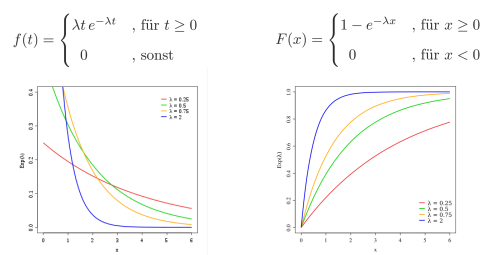
\includegraphics[width=0.9\linewidth]{images/exponential-verteilung.png}
\end{minipage}

\textbf{Anwendung/Beispiele}
\begin{itemize}
        \item Zeitspanne zwischen zwei Anrufen in einer Telefonzentrale.
        \item Dauer eines Telefongesprächs. 
        \item Lebensdauer eines Geräts, wenn Defekte durch äußere Einflüsse und nicht durch Verschleiß verursacht werden (ansonsten Weibulverteilung) 
\end{itemize}

\textbf{Berechnungen} \\
\textit{Interarrivalzeit / Rate}
\begin{flalign*}
\lambda
\end{flalign*}
\textit{(Median (50\% Perzentil):)}
\begin{flalign*}
Median = \frac{ln(2) }{\lambda}  = 0.693
\end{flalign*}
\textit{Modus:}
\begin{flalign*}
0
\end{flalign*}
\textit{Varianz:}
\begin{flalign*}
Var(X) = \sigma^2 = \frac{1}{\lambda^2}
\end{flalign*}

\subsection{Normalverteilung}
Wieso spielt die Normalverteilung in der Simulation keine Rolle?
\\
Weil negative Werte möglich sind, welche in einer Simulation nicht verwendet werden können
\subsection{Erzeugen von Zufallszahlen}
Für Simulationsexperimente werden Zufallszahlen gebraucht. 
\\
Die Zufallszahlen haben folgende Eigenschaften:
\begin{itemize}
    \item Die Zufallszahlen müssen einer bestimmten Verteilungsfunktion folgen
    \item Die Zufallszahlen müssen eindeutig in der Folge ihres Auftretens sein
    \begin{itemize}
        \item Die Experimente sind daher unter exakt gleichen Bedingungen wiederholbar
    \end{itemize}
    \item Es müssen beliebig viele dieser Zufallszahlen generiert werden können
    \begin{itemize}
        \item um verschiedenen Prozessen ein unterschiedliches Verhalten zu geben
        \item um unterschiedlichen Experimente machen zu können
    \end{itemize}
\end{itemize}

Aus den oben genannten Eigenschaften/Gründen ist ersichtlich, dass keine \textit{echten} Zufallszahlen verwendet werden können. Diese sind nämlich nicht reprodzierbar und haben oft schlechte statistische Eigenschaften (nicht true random).
\\
Als Lösung werden sogenannte Pseudo-Zufallszahlen verwendet. Diese haben folgende passende Eigenschaften:
\begin{itemize}
    \item Folgen einer Gesetzesmässigkeit und sind daher wiederholbar
    \item Besitzen gute statistische Eigenschaften
    \item Können einfach und schnell für verschiedene Verteilungsfunktionen erzeugt werden
\end{itemize}

\section{Prinzipien der Prozessverbesserung}
\subsection{Grundlagen}
Ein System besteht aus einer Reihe von sequentiellen und parallelen Prozessen und den Transportwegen zwischen den Prozessen. Die Prozessausgestaltung entscheidet unter anderem über:
\begin{itemize}
    \item den erreichbaren Durchsatz
    \item die durchschnittliche Zeit von Jobs im System
    \item der Anzahl des WIP (workin process)
    \item Die Utilization
    \begin{itemize}
        \item der Prozessressourcen
        \item der Transportressourcen
    \end{itemize}
\end{itemize}

Nun gibt es verschiedene Möglichkeiten, wie eine Prozessverbesserung erreicht werden kann.
Man kann Veränderungen an folgenden Elementen vornehmen:
\begin{itemize}
    \item Die Prozessgrössen 
    \begin{itemize}
        \item Varianz, Reise-, Rüst-und Servicezeiten
        \item Puffergrössen
    \end{itemize}
    \item Die Zugriffsstrategie auf das Inputsystem 
    \begin{itemize}
        \item push
        \item pull
    \end{itemize}
    \item Die Zugriffsstrategie auf den Inputbuffer
    \begin{itemize}
        \item FIFO, LIFO, ShortestJob first,
    \end{itemize}
    \item Die Prozessreihenfolge (falls es möglich ist zu varrieren), wo:
    \begin{itemize}
        \item sollte der schnellste Prozess platziert werden?
        \item der Prozess mit der höchsten Varianz platziert werden?
    \end{itemize}
\end{itemize}

\subsection{Allgemeine Regeln}
Nun lassen sich einige allgemeine Regeln für die Prozessoptimierung festlegen.
\newline

\textbf{Variation verringert die Performance} 
\newline
Variation drückt sich messbar in der Varianz eines Arbeitsschrittes aus. Sie wird erzeugt durch zufällige Änderungen in einem Prozess, z.B. im Bearbeitungsprozess, im Bestellprozess oder im Lieferprozess.
Ziel ist es also die Variation möglichst klein zu halten. Dafür muss folgendes gemacht werden:\\
\newline
 Suche Quellen im System, die Variation (Varianz) verursachen und eliminiere sie. \\
 \newline
 
 \textbf{Utilization erhöht die Work in Process }
 \newline
 Ist die Utilization hoch, so ist auch der Work in Process hoch. Beide Werte gehen Hand-in-Hand. Somit kann folgende Regel festgelegt werden: \\
 \newline
 Vermeiden Sie es, einen zu hohen WIP zu erzeugen, indem Sie die Utilizationder Ressource unnötig erhöhen. \\
 \newline 
 
 \textbf{Reduktion der WIP - Single Queue statt Multiple Queue }
 \newline
 Eine Reduktion des Work in Process kann beispielsweise erreicht werden, indem man eine Single Queue statt eine Multi Queue verwendet. Aus der Theorie der Warteschlange geht hervor, dass die Residenzzeit eines Systemes kleiner ist, wenn nur eine Warteschlange mit \textit{n} Server, anstatt für jeden Server eine eignene Warteschlange verwendet wird.  Somit kann folgende Regel festgelegt werden: \\
 
 Benutze eine einzelne Warteschlange vor mehreren Servern!\\
 \newline
 
\textbf{Reduktion der WIP - Shortest Processing first }
\newline
Nicht jeder Job hat die gleiche Bearbeitungszeit. Jobs werden üblicherweise nach dem FIFO-Prinzip abgearbeitet.
Ist die WIP zu optimieren, so ist es intuitiv, zuerst die kurzen Jobs zu bearbeiten.
So wird auch hier die Regel festgelegt:\\
Wenn der WIP zu reduzieren ist, dann bearbeite zuerst kurze Jobs.\\
 \newline

\textbf{CONWIP - Constant quality of Work in Progress }
\newline
Um ein optimales Ergebnis zu erreichen, sollte ein Pull- einem Push-Ansatz vorgezogen werden.
Ein Pull wird ausgelöst, wenn die Anzahl der definierten WIP unterschritten ist.
Der optimale Work in Progress wird z.B durch Simulation bestimmt. So kann auch hier eine Regel festgehalten werden: \\
\newline
Verwende, wo möglich, einen Pull-Ansatz
\newline

\section{Model Verification and Validation  }
In diesem Kapitel wird die Modell Verifikation und Validierung vertieft angeschaut.

\begin{minipage}[t]{0.9\textwidth}
\centering
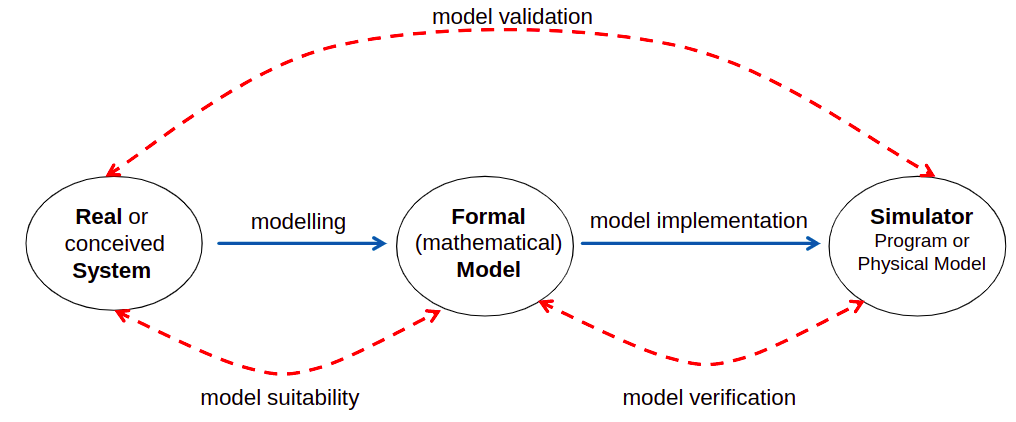
\includegraphics[width=0.9\linewidth]{images/simulationsphasen.png}
\end{minipage}

\subsubsection{Warum Verifikation und Validierung}
Simulation ist sehr komplex und es fallen mehrere Diziplinen zusammen: 
\begin{itemize}
    \item Experimentenplanung und -durchführung inkl. der Auswertung
    \item Modellbildung und Spezifikation, dafür ist Methoden- und Domänenwissen erforderlich
    \item Implementierung des Modells - dafür müssen die entsprechenden Tools (\& SW-Engineering) beherrscht werden
\end{itemize}

Die Simulation hängt stark von zwei Schritten ab:
\begin{enumerate}
    \item Wurde das spezifizierte Modell korrekt umgesetzt? - Verifikation 
    \item Wurde das richtige Modell im Bezug auf die Fragestellung gebaut? - Validierung  
\end{enumerate}

\subsubsection{Verifikation}
Die Verifikation untersucht die Frage, ob das Modell gegenüber seiner Spezifikation richtig implementiert wurde.

\textit{Je präziser (formaler) die Beschreibung (Spezifikation), desto besser oder leichter ist
die Verifikation bzw. desto verlässlicher ist der Test}


Folgende Punkte sind also wichtig:
\begin{itemize}
    \item Das konzeptionelle Modell, gegeben durch seine Spezifikation, muss verglichen werden mit der Computerimplementierung (am besten automatisch)
    \item Die folgende Punkte müssen eindeutig überprüft, werden:
    \begin{itemize}
        \item Ist die Architektur korrekt implementiert, d.h alle Koponenten und deren Kommunikationsbeziehung
        \item Sind alle Inputparameter korrekt eingestellt
        \item Ist das logische Verhalten, die Regeln, hinsichtlich der Spezifikation richtig implementiert
        \item Ist der Fluss von Entitys durch das System korrekt
    \end{itemize}
\end{itemize}
\newline

\textbf{Beispiele}
\begin{itemize}
    \item Ist in der Simulation der Input Buffer der Maschine 1 auf 4 gestellt.
    \item Ist in der Simulation die Stapler Geschwindigkeit auf 10km/h eingestellt.
    \item Ist in der Simulation die spezifizierte Verteilungsfunktion richtig konfiguriert .
\end{itemize}
\newline

\textbf{Ansätze/Methoden}
\begin{itemize}
    \item Möglichst selbsterklärender (gut dokumentierter) Code 
    \item Test durch Testteams durch führen lassen, nicht durch die Entwickler 
    \item Testen der einzelnen Komponenten (Unit-Tests), „Teile und Herrsche“ 
    \item Testen von Randwerten, Systemgrenzen 
    \item Erstellen von Testszenarien als fester Bestandteil der Implementierung 
\end{itemize}
\info{Problem}{Viele Testergebnisse, wie beispielsweise die Utilisation, die Durchlaufzeiten, die Aufteilungen des Entityflusses, werden statistischen Schwankungen unterliegen, dies macht ein statistisches Testen unumgänglich.}
 
\subsubsection{Validierung}
Beschäftigt sich mit der Frage, ob das System hinsichtlich des zu untersuchenden Fragebereichs
richtig abgebildet wurde: \\

\textit{Verhält sich das Modell so wie das Original?}
\newline

\textbf{Ansätze/Methoden} \\
\newline
Die Validierung kann erreicht werden mit:
\begin{itemize}
    \item Kalibrieren des Modells, hierbei ist die gesamte Architektur, inklusive Datenmarerial zu berücksichtigen. Dabei handelt es sich um:
    \begin{itemize}
        \item um einen iterativen Prozess des Vergleichs zwischen dem erstellten Modell und dem realen System
        \item um einen Lernprozess, wie das reale System funktioniert und in seinen Komponenten wechselwirkt 
    \end{itemize}
    \item Diese Kalibrierung wird solange durchgeführt, bis eine hinreichende Genaugikeit erreicht wurde
\end{itemize}
\info{Gefahr}{Bloßes „tunen“ von Einstellungen (ohne Verständnis der Wirkzusammenhänge), bis ein gewünschtes Ergebnis erreicht wird. Die Gefahr ist umso grösser, je kleiner der zur Verfügung stehende Datenumfang zur Validierung ist \to Scheinvalidierung }

\textbf{Vorgehensweis zur Validierung von Naylor and Finger} \\
\newline
\begin{minipage}[t]{0.\textwidth}
\centering
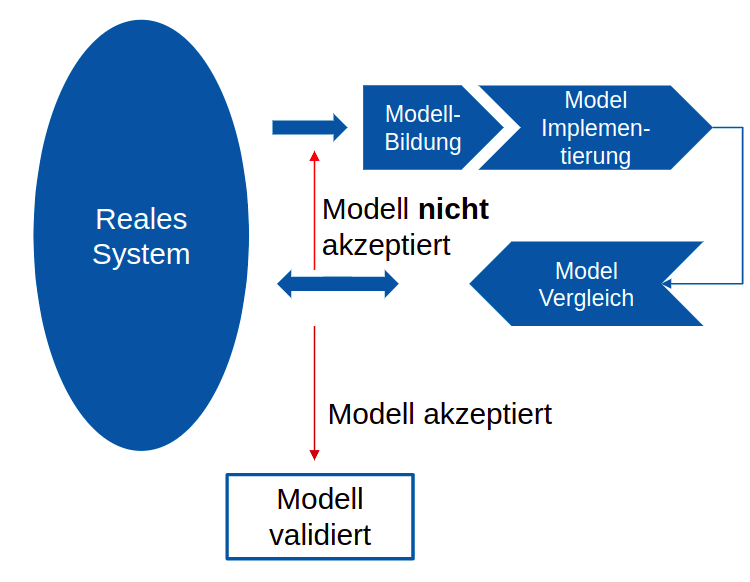
\includegraphics[width=0.9\linewidth]{images/ansatz-der-validierung.png}
\end{minipage}
Die Vorgehensweis zur Validierung von Naylor and Finger besteht aus drei Schritten:
\begin{enumerate}
    \item Bilden eines strukturellen Models
    \item Validierung des Modells (und der Modellannahmen - Model Assumptions )
    \item Vergleichen des Modells mit dem realen System (input-output Transformationen)
\end{enumerate}


\textit{1. Bilden eines strukturellen Models}

\begin{itemize}
    \item Wie ist die Architektur des Systems? 
    \item Wie arbeitet das Modell (Logik)?
    \item Wie verläuft der Entity-fluss durch das System? 
\end{itemize}
Das strukturelle Model kann sehr gut visualisiert/animiert werden (z.B an einem Dashboard)
\info{face validity}{\textit{face validity}meint die subjektive Bestätigung durch die Experten }
\newline


\textit{2.  Validierung des Modells (und der Modellannahmen - Model Assumptions )}

\info{Datenannahmen}{Datenannahmen (Data/Model Assumptions) sollten auf der Basis von Messdaten und statistischer Standards zur Erhebung erfolgen - empirische Daten }
\newline 
Die anschliessende Analyse der empirischen Eingangsdaten erfolgt grob in drei Schritten:
\begin{enumerate}
    \item Identifizieren der geeigneten Wahrscheinlichkeitsdichtefunktion 
    \item Schätzen der erforderlichen Parameter der theoretischen Funktion 
    \item Validieren des statistische Modells durch einen Test
\end{enumerate}
\\
\info{Problem}{Folgende Problem treten dabei auf: 
\begin{itemize}
    \item Die Autokorrelation der Daten wir meist durch diese Tools nicht berücksichtigt
    \item die Generatoren von Zufallszahlenfolgen sind meist Autokorrelationsfrei
    \item Empirische Daten besitzen jedoch oft eine Autokorrelation ungleich null, das kann zu nicht validen Modellen führen.
\end{itemize}}
\newline


\textit{3. Vergleichen des Modells mit dem realen System (input-output Transformationen)}\\
\newline 
Sind die Werte zweier Modelle zu vergleichen, so ist ein Differenztest durchzuführen.
Bei der Modellvalidierung  sollte die Gleichheit der Modelle nachgewiesen werden.
\newline 

\section{Experimentierplan und Optimierung}
\subsection{Wieso werden Versuche/Experimente benötigt?}
\begin{itemize}
    \item Produkte und Fertigungsprozesse müssen ständig verbessert werden, egal durch Simulation oder am Original 
    \item Der Funktionsumfang der Produkte muss erhöht werden. Die Anforderungen der Kunden müssen immer besser erfüllt werden. 
    \item Die Kosten müssen gesenkt werden, z. B. durch geringere Materialkosten oder höhere Ausbeute. 
    \item Die Entwicklungszeit neuer Produkte und ihre Durchlaufzeit in der Fertigung müssen immer weiter verkürzt werden. 
\end{itemize}

Um dies zu erreichen muss man verschiedene Zusammenhänge untersuchen. Mittels gezielten Experimenten können diese einzelnen Daten untersucht werden. Anhand der ermittelten Daten können dann Rückschlüsse für Verbesserungen gezogen werden.

\subsection{Begriffe}
\subsubsection{Zielgrössen}
Zielgrößen beschreiben das Ergebnis eines Versuch. Im Simio wurden diese als \textit{Responses} gekenntzeichnet. Können Messwerte oder daraus berechnete Grössen sein. Bei einem Versuch können mehrere Zielgrössen definiert werden.
\subsubsection{Einflussgrössen}
Einflussgrößen sind Größen, die die Versuchsergebniss, die Zielgrößen, möglicherweise beeinflussen und teilen sich auf in:
\begin{itemize}
    \item Steuergrössen - im Simio \textit{controls}
    \begin{itemize}
        \item könne auf einen bestimmten Wert eingestellt werden, können beeinflusst werden
    \end{itemize}
    \item Störgrößen
    \begin{itemize}
        \item Störgrößen sind Einflussgrößen, deren Wert für das Produkt bzw. den  Prozess nicht vorgegeben werden kann (zT unvorhersehbar)
    \end{itemize}
\end{itemize}
\subsubsection{Faktoren}
Aus der Vielzahl der Einflussgrößen werden für das Experiment die vermuteten wesentlichen Einflussgrößen, die Faktoren, ausgewählt

\subsubsection{Faktorstufen}
Nach der Auswahl der Faktoren muss festgelegt werden, welche Werte die Faktoren im Experiment annehmen sollen, diese Werte werden Faktorstufen genannt. Diese werden unterteilt in:
\begin{itemize}
    \item Quantitative Faktoren - die Stufen werden mit Zahlenwerte einer Messkala beschrieben
    \item Qualitative Faktoren - Namen, Beschreibungen, Bezeichnungen
\end{itemize}

\subsection{Vorgehensweise - Design of Experiments}

Bei der Vorgehensweise wird auf das DoE-Prinzip (Design of Experiments) verwiesen.

\begin{minipage}[t]{0.9\textwidth}
\centering
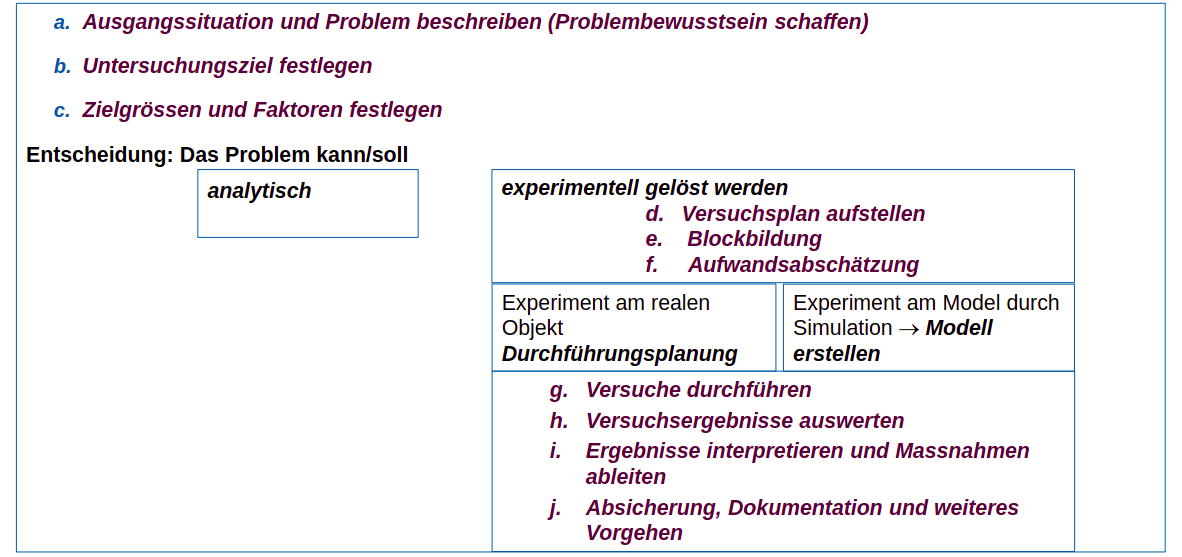
\includegraphics[width=0.9\linewidth]{images/doe.png}
\end{minipage}

\subsubsection{Ausgangssituation und Problem beschreiben (Problembewusstsein schaffen)}
Bei diesem Schritt werden grundlegende Fragen gestellt und beantwortet wie:
\begin{itemize}
    \item Wer ist der Kunde? 
    \begin{itemize}
        \item Wer ist der Konkurrent?  
        \item Was braucht der Kunde? 
        \item Was ist die Verbesserung wert? 
    \end{itemize}
    \item Was ist die langfristige Zielsetzung? 
    \item Welches (Teil-)Problem soll durch die geplante Untersuchung gelöst werden? 
    \begin{itemize}
        \item Teile und Herrsche
        \item Abstrahiere hin zum Wesentlichen, isolierende Abstraktion
        \item Nur so genau wie nötig NICHT wie möglich! 
    \end{itemize}
    \item Wie viel Zeit und Geld stehen maximal zur Verfügung? 
    \begin{itemize}
        \item Kosten-Nutzen-Analyse erforderlich
    \end{itemize}
    \item Wer ist von der geplanten Untersuchung betroffen 
    \begin{itemize}
        \item Sind alle eingebunden? 
        \item Ist mit Widerständen zu rechnen, 
        \item Wer ist Wissensträger?
        \item Wer profitiert/verliert? 
    \end{itemize}
    \item Wer ist für das Projektmanagement verantwortlich?
    \item Was ist über das zu untersuchende Problem bereits bekannt? 
    \item Liegen bereits (aktuelle) Daten vor? 
\end{itemize}

\info{Zentrale Frage}{So stellt sich die entscheidene Zentrale Frage: \textit{Ist das Problem wirklich verstanden? }}

\subsubsection{Untersuchungsziele des DoE festlegen }
In einem nächsten Schritt sollte man die Untersuchungsziele festlegen. Dieser Schritt beinhaltet punkte wie:
\begin{itemize}
    \item \textbf{Optimale Lage des Mittelwerts} - das Prozessergebnis oder ein Produktparameter sollen einen bestimmten Wert annehmen 
    \item \textbf{Reduzierung der Streuung/Robustheit} - oft ist weniger die Lage des Mittelwerts des Prozessergebnisses problematisch als dessen Streuung 
    \item \textbf{Erkennen der wichtigsten Störgrössen} (in der Fertigung) durch systematische Beobachtung (der Fertigung) und einfache Versuche herausfinden 
    \item \textbf{Verbesserungsmöglichkeiten erkennen} - Lernen durch systematische Veränderung der Prozessparameter innerhalb ihrer Spezifikation in den laufenden Prozess (Fertigung)
    \item \textbf{Funktion und Zuverlässigkeit} nachweisen
    \item \textbf{Weitere Fragen} z.B bezüglich KPI (Key Perfomance Indicators) in der Simulation
\end{itemize}

\subsubsection{Zielgrössen festlegen}
In einem nächsten Schritt sollte man zusammen mit dem Kunden die Zielgrössen festlegen. Man definiert die Werte, welche der Kunde gerne haben will:
\begin{itemize}
    \item \textbf{Kundenorientiert und Relevant} - Zielgrössen müssen die Probleme des Kunden abbilden und zielorientiert sein
    \item \textbf{Messbar} - Zielgrössen müssen quantifizierbare bzw. messbare Grössen sein
    \item \textbf{Vollständigkeit} - Alle wesentlichen Prozessergebnisse bzw. Produkteigenschaften müssen als Zielgrössen erfasst werden, nicht nur die momentan problematischen Grössen berücksichtigen!
    \item \textbf{Verschiedenheit} - Die Interpretation der Ergebnisse wird erleichtert, wenn die Anzahl der Zielgrössen möglichst klein ist und jede Zielgrösse einen anderen, möglichst grundlegenden Zusammenhang erfasst
\end{itemize}

\info{Best Practice}{Die Auswahl der Zielgrössen erfolgt in zwei Schritten:
\begin{enumerate}
    \item erst möglichst viele (alle) Einflussgrössen sammeln 
    \begin{itemize}
        \item Prozessablaufdiagramme (Flussbild), Objektdiagramme, Zustandsdiagramme (UML, SysML, BPMN, ..) 
        \item Ursache-Wirkungsdiagramme (System Dynamics, Fischgrätendiagramme), 
        \item Tabellen z.B. Einflussgrössen-Zielgrössen-Matrix 
        \item Text, Erläuterungen, etc.
    \end{itemize}
    \item danach auf eine handhabbare Anzahl von Faktoren (die wichtigsten) reduzieren 
\end{enumerate}}

\subsubsection{Faktoren und Faktorstufen festlegen}
Nachdem die Zielgrössen gefunden worden sind, müssen die Faktoren festgelegt sein. Um Faktoren und deren Faktorstufen festzulegen, müssen zuerst Faktoren gefunden werden und dann isoliert werden:
\begin{enumerate}
    \item  Abschluss der Ideenfindung werden die Ideen bewertet und gewichtet
    \item Personen mit Expertenwissen wählen einige (typisch 3-6) unabhängige Faktoren der gefundenen Einflussgrössen aus (Isolierung)
    \item Faktorenstufen festlegen
\end{enumerate}
\newline

Bei der Wahl der \textbf{Faktorenstufen} sollte auf folgendes geachtet werden:
\begin{itemize}
    \item je kleiner der Abstand zwischen den Stufen ist, desto kleiner der Unterschied der Ergebnisse 
    \item Kann ein Faktor nicht genau gemessen werden, so sollte der Abstand der Faktorstufen mindestens 6 x so gross wie die Standardabweichung sein 
    \item Die Untersuchung den interessanten/relevanten Bereich enthalten. 
\end{itemize} 

\subsection{Versuchsplan}
Beim Versuchsplan sollte auf folgendes ein Augenmerk gelegt werden:
\begin{itemize}
    \item Nicht zu viele Realisierungen pro Versuch
    \item Minimierung der Zufalsstreuung mittels Einteilung der Einzelversuche bzw. Versuchsobjekte in Gruppen (Blockbildung)
    \begin{itemize}
        \item Somit sind die zufälligen Unterschiede pro Block möglichst klein
        \item Somit tritt jede Faktorstufenkombination möglichst gleich häufig auf
    \end{itemize}
    \item Randomisierung - verhindert, dass ein Trend oder eine andere unerkannte Änderung der Ergebnisse die Schätzung der Effekte der Faktoren verfälscht. 
    \begin{itemize}
        \item Zufällige Reihenfolge bedeutet nicht beliebige Reihenfolge 
        \item Die Reihenfolge wird durch Zufallszahlen pro Block bestimmt 
    \end{itemize}
    
    
\end{itemize}


\part{Cheatsheet}

\section{Theoriefragen}
\begin{itemize}
    \item Simulation experimentell oder analytisch?
    \begin{itemize}
        \item Experimentell
    \end{itemize}
    \item Was ist dynamische Simulation?
    \begin{itemize}
        \item Die Zeit spielt eine Rolle.
    \end{itemize}
    \item Was ist eine diskrete Systemänderung
    \begin{itemize}
        \item Der Zustand ändert sich diskret zu einem bestimmten Zeitpunkt.
    \end{itemize}
    \item Was ist stochastische Simulation?
    \begin{itemize}
        \item Ereignisse treten zufällig ein?
    \end{itemize}
    \item Begriff der Generalisation / generalisierender Abstraktion?
    \begin{itemize}
        \item Signifikante Parameter werden variabel gemacht
    \end{itemize}
    \item Begriff der Isolation / isolierende Abstraktion
    \begin{itemize}
        \item Es werden nur die Systemparameter und –Komponenten berücksichtigt, die zur Beantwortung der Fragestellung benötigt werden.
    \end{itemize}
    \item Begriff der Validierung?
    \begin{itemize}
        \item  Ob das Modell dem zur beantwortung der Fragen dem Realsystem entspricht.
        \item Gültigkeitserklärung des Modells als Abbildung des Realsystems hinsichtlich der zu beantwortenden Fragen.
    \end{itemize}
    \item Begriff der Verifikation?
    \begin{itemize}
        \item Nachweis/Beweis, dass die Simulation der Spezifikation oder dem Modell entspricht

    \end{itemize}  
     \item Warum mehrere Simulationsdurchläufe?
    \begin{itemize}
        \item Weil die Ergebnisse um einen Mittelwert schwanken, da Simulation ein exp. Verfahren.
        Damit das Ergebnis signifikat wird, müssen viele Experimente durchgeführt werden.
    \end{itemize}  
    \item Was ist das Dualitätsprinzip?
    \begin{itemize}
        \item Die Unterscheidung zwischen der Modellzeit und der zur Ausführung erforderlichen Rechenzeit.
        \item Das Weiterstellen der Simulationszeit benötigt keine Rechenzeit.
        \item Das Abarbeiten der Ereignisse benötigt zwar Rechenzeit, aber keine Simulationszeit.
    \end{itemize}  
     \item Unterschied zwischen SysML und UML?
    \begin{itemize}
        \item Klassen sind Blöcke
        \item Parts sind Properties als Instanz der Blöcke
        \item Objekte sind Instance Specification-Elemente
        \item Darstellung als Block und Subblockdiagramme mit Flow Ports und Item Flow
    \end{itemize}  
     \item Was ist das seed bei Pseudozufallszahlen?
    \begin{itemize}
        \item Es ist die "Keimzahö" aus dem die Zufallszahlenfolge generiert wird
    \end{itemize}  
     \item Wozu kann man das Seed benutzen?
    \begin{itemize}
        \item Um unterschiedlichen Zufallszahlenfolgen gleicher Verteilung zu generieren.
    \end{itemize} 
     \item Wie kann man mit gleichverteilten Zufallszahlen, Zufallszahlen anderer Verteilungen erzeugen?
    \begin{itemize}
        \item Mit Hilfe der Umkehrfunktion.
    \end{itemize} 
    \item Was versteht man unter dem Begriff des Eingeschwungenen Zustandes?
    \begin{itemize}
        \item Wenn der Mittelwert konstant bleibt
        \item Je länger das System simuliert wird, desto näher ist es am Eing. Zustand.
        \item Kann mathematisch mit Hilfe von Warteschlangen, Durchlaufzeiten etc. berechnet werden
    \end{itemize} 

\end{itemize}

\section{Berechnungen}



\begin{minipage}{0.45\textwidth}
    \begin{description}
    \item[A:] Anzahl der ankommenden Token
    \item[T:] Beobachtungszeit des Systems
    \item[C:] Anzahl der abgefertigten Token
    \end{description}
\end{minipage}
\begin{minipage}{0.45\textwidth}
    \begin{description}
    \item[B:] aktive Systemzeit \textit{(busy time)}
    \item[T:] Beobachtungszeit des Systems
    \item[W:] Waiting Time
    \end{description} 
\end{minipage}
\newline
\newline
\newline


\begin{minipage}{0.45\textwidth}
    \begin{description}
        \item[Utilization\footnote{Bei der Utilization gelten die letzen zwei Formeln nur wenn das System stabil ist.}:] $U = \frac{B}{T} \Longleftrightarrow S \cdot X 
        \Longleftrightarrow S \cdot \lambda $ 
        \item[Arrival Rate:] $\lambda = \frac{A}{T}$
        \item[Service Time:] $ S = \frac{B}{C}$
        \item[Number in Queue:] $ N_Q = \lambda \cdot W  \Longleftrightarrow N_Q = \frac{U}{1-U} $
        \item[Waiting Time: ] $W = \frac{S \cdot U}{1-U} $
    \end{description}
\end{minipage}
\begin{minipage}{0.45\textwidth}
    \begin{description}
        \item[Durchsatz:] $X = \frac{C}{T} $
        \item[Residence Time:]$R = W + S $ $\Longleftrightarrow$ $\frac{S}{1 - \lambda S}$
        \item[Number in System\footnote{Bei der Number in System giltet die zweite Formel nur im stabilen System}:] $ N = \lambda \cdot R  \Longleftrightarrow N = X \cdot R $ 
        \item[Stabiles System] $N = N_Q + U \Longrightarrow \textbf{U < 1} $
        \item
    \end{description}  
\end{minipage}

\info{U > 1}{Ist bei einer Maschine die Utilization grösser 1 so wird diese Maschine zur Quelle. Es muss also mit U = $\lambda$ * S weitergerechnet werden}

\section{Utilization berechnen Beispiel}
\subsection{Gegeben}
\begin{itemize}
    \item Zwei verschiedene Arten von Pralinen: Nusspralinen und Marzipanpralinen
    \item Marzipanpralinen kommen im Durchschnitt alle 12 Sekunden (gleichverteilt 11,13)
    \item Nusspralinen kommen im Durchschnitt alle 8 Sekunden (gleichverteilt 7,9)
    \item Prozess
    \begin{enumerate}
        \item Schokoladenüberzug dauert zwischen 4 und 5 Sekunden
        \item Kontrolle 2 Sekunden, 10\% der Pralinen müssen nachbearbeitet werden
        \item Nusspralinen erhalten Nuss und dann Verpackt, Marzipanpralinen direkt verpack
        \item Verpacken dauert durchschnittlich 12 Sekunden (mind. 10s und max. 14s) - es hat 3 Verpackungsmaschinen
    \end{enumerate}
\end{itemize}

\subsection{Gesucht}
\begin{itemize}
    \item Auslastung (Utilization) der Maschinen
\end{itemize}

\subsection{Vorgehen}
\subsubsection{Gesamtrate berechnen}
Die Gesamtrate ergibt sich aus der Addition der Nuss- und der Marzipanpralinenrate.
\begin{flalign*}
   \lambda_G= \lambda_N + \lambda_M = \frac{1}{8} + \frac{1}{12} = \frac{5}{24} = 0.21
\end{flalign*}
\subsubsection{Effektive Rate berechnen}
Da 10\% der Pralinen zurückgehen, muss dies beachtet werden und die effektive Rate berechnet werden:
\begin{flalign*}
   \lambda_E = \frac{\lambda_G}{1 - p}  = \frac{0.21}{1 - 0.1 } = \frac{0.21}{0.9 } = 0.23 
\end{flalign*}

\subsubsection{Utilization Schokoladenüberzug berechnen}
Nun muss die Utilization des Schokoladenüberzugs berechnet werden, dafür brauchen wir die Effektive Utilization (0.23) und die Servicezeit (7s im Durchschnitt).
\begin{flalign*}
   U_S = \lambda_E * S_S = 0.23 * 4 = 0.926
\end{flalign*}

\subsubsection{Utilization Kontrolle berechnen}
Die Kontrolle dauer 2 Sekunden und kann analog zum Schokoladenüberzug berechnet werden.
\begin{flalign*}
   U_K = \lambda_E * S_K = 0.23 * 2 = 0.463
\end{flalign*}

\subsubsection{Utilization Nussmaschine berechnen}
Bei der Nussmaschine kommen nur die Nusspralinen an, deshalb muss hier mit der Nuss-Rate gerechnet werden. Die Zeit ist nicht angegeben als 1:
\begin{flalign*}
   U_N = \lambda_N * S_N = \frac{1}{8} * 1 = 0.125
\end{flalign*}

\subsubsection{Utilization Verpackung berechnen}
Bei der Verpackung muss mit der gesamten Rate (5/24) gerechnet werden, da irgendwann jede Praline verpacket wird. Ebenfalls muss die Verpackungszeit einberechnet(12s) werden. Es darf nicht vergessen werden, dass 3 Maschinen vorhanden sind:
\begin{flalign*}
   U_V = \frac{\lambda_E * S_V}{Anzahl Maschinen} = \frac{\frac{5}{24} * 12}{3} = 0.8333
\end{flalign*}

\section{Maximale Servicezeit bei gegebener Wartezeit berechnen}
\subsection{Gegeben}
\begin{itemize}
    \item Durchschnittliche Ankunftsrate 1 Kunde Pro 3 min --> $\lambda = \frac{1}{3}$ (0.333)
    \item Durchschnittliche Wartezeit von 4 min darf nicht überschritten werden
\end{itemize}

\subsection{Gesucht}
\begin{itemize}
    \item Maximale Servicezeit, dass die Wartezeit von 4 min nicht überschritten wird.
\end{itemize}

\subsection{Vorgehen}
\subsubsection{Intervallrate Berechnen}
Die Rate kann anhand der gegebenen Wartezeit W und der Ankunftsrate $\lambda$ bestimmt werden.
\begin{flalign*}
   W= \frac{\lambda}{\mu(\mu - \lambda)} = 4
\end{flalign*}

Somit kann eine Quadratische Gleichung aufgestellt werden, welche mit der Mitternachtsformel aufgelöst werden kann:

\begin{flalign*}
4\mu^2 - 1.332\mu - 0.333 = 0
\end{flalign*}

Daraus ergibt sich:

\begin{flalign*}
x\textsubscript{1} = -0.13 \textbf{ kann nicht negativ sein}
\end{flalign*}
\begin{flalign*}
x\textsubscript{2} = 0.49 \approx \mu \textbf{= 0.5}
\end{flalign*}
\subsubsection{Servicezeit berechnen}
Die Servicezeit kann anhang der berechneten Intervallrate berechnet werden:

\begin{flalign*}
\mu = \frac{1}{S}
\end{flalign*}

S ist Somit:
\begin{flalign*}
S = \frac{1}{\mu}
\end{flalign*}

Die Servicezeit darf maximal \textbf{2 Minuten} betragen

% Anhänge / Infos einfügen
\appendix

% Code Listings
\lstlistoflistings

% List of figures
\listoffigures

% List of tables
\listoftables

% Bibliography
\bibliographystyle{plain} 
\bibliography{literatur}

\end{document}